%%%%%%%%%%%%%%%%%%%%%%%%%%%%%%%%%%%%%%%%%%%%%%%%%%
%% Bachelor's & Master's Thesis Template        %%
%% Copyleft by Dawid Weiss & Marta Szachniuk    %%
%% Faculty of Computing and Telecommunication   %%
%% Poznan University of Technology, 2020        %%
%%%%%%%%%%%%%%%%%%%%%%%%%%%%%%%%%%%%%%%%%%%%%%%%%%


% Szkielet dla pracy licencjackiej pisanej w języku polskim.

\documentclass[polish,bachelor,a4paper,oneside]{ppfcmthesis}


\usepackage[utf8]{inputenc}
\usepackage[OT4]{fontenc}

%--------------------------------------
% Strona tytułowa
%--------------------------------------

% Autorzy pracy, jeśli jest ich więcej niż jeden
% wstaw między nimi separator \and
\author{%
   Jagoda Janowska \album{151798} \and 
   Adam Maciejak \album{151756} \and
   Adam Mikołajczak \album{151247}}
\authortitle{}                                % Do not change.

\title{Zastosowanie dużego modelu językowego \\do generowania modeli programowania liniowego \\ze słownych opisów problemów optymalizacyjnych}

% Your supervisor comes here.
\ppsupervisor{dr hab.~inż.~Tomasz Pawlak} 

% Year of final submission (not graduation!)
\ppyear{2025}                                 


\begin{document}

% Front matter starts here
\frontmatter\pagestyle{empty}%
\maketitle\cleardoublepage%

%--------------------------------------
% Miejsce na kartę pracy dyplomowej
%--------------------------------------

\thispagestyle{empty}\vspace*{\fill}%
\begin{center}Tutaj będzie karta pracy dyplomowej;\\oryginał wstawiamy do wersji dla archiwum PP, w pozostałych kopiach wstawiamy ksero.\end{center}%
\vfill\cleardoublepage%

%--------------------------------------
% Spis treści
%--------------------------------------

\pagenumbering{Roman}\pagestyle{ppfcmthesis}%
\tableofcontents* 
\cleardoublepage % Zaczynamy od nieparzystej strony

%--------------------------------------
% Rozdziały
%--------------------------------------

%Najwygodniej jeśli każdy rozdział znajduje się w oddzielnym pliku
\mainmatter%

\chapter{Wprowadzenie}\label{ch:intro}

\section{Motywacja}\label{sec:intro:motivation}

Programowanie Liniowe \english{Linear Programmimng, PL} jest popularną metodą modelowania zagadnień optymalizacyjnych, szczególnie w badaniach operacyjnych \cite{williams2013model}. PL ma liczne zastosowania, np.~w logistyce, planowaniu łancuchów dostaw oraz optymalizacji zużycia materiałów.\cite{dantzig2002linear} % TP: no ok, ale oryginalne prace Dantziga są z lat 1940... - DONE
% TP: rozszerzam motywację o niezbędne elementy
Model PL składa się ze zmiennych odpowiadających zmiennym czynnikom modelowanego zagadnienia i~specyfikowanych wraz z~dziedzinami (ciągłe, całkowitoliczbowe, z określonego przedziału); ograniczeń wyrażających cechy zagadnienia w~kategoriach zależności liniowych pomiędzy zmiennymi; funkcji celu określającej pożądane cechy rozwiązania jako funkcję liniową zmiennych. Na potrzeby tej pracy, definicję modelu PL rozszerzono o~zbiory wartości odpowiadające wymiarom modelowanego zagadnienia oraz parametry odpowiadające stałym wartościom liczbowym. Są to czynniki umożliwiające wysokopoziomowy zapis modelu w~abstrakcji od wartości liczbowych występujących w konkretnej instancji zagadnienia. Wówczas implementację modelu PL dla konkretnej instancji realizuje się poprzez podstawienie wartości pod zbiory i~parametry.
Wektor wartości zmiennych nazywany jest \emph{rozwiązaniem} modelu PL. Rozwiązanie jest \emph{dopuszczalne} jeśli spełnia wszystkie ograniczenia. Rozwiązanie dopuszczalne jest \emph{optymalne}, jeśli minimalizuje lub maksymalizuje funkcję celu.

Do rozwiązywania modeli PL istnieje wiele solverów, zarówno komercyjnych takich jak Gurobi\cite{gurobi2023} czy CPLEX\cite{cplex2019}, jak i otwartoźródłowych, takich jak GLPK\cite{glpk2023}, COIN-OR CBC\cite{cbc2023} oraz SCIP\cite{scip2023}. %Solvery rozwiązują modele programowania liniowego, które mogą być zapisane za pomocą różnych języków programowania z ograniczeniami. 
Korzystanie z solwerów jest do pewnego stopnia ustandaryzowane dzięki wsparciu dla wysokopoziomowych języków zapisu modeli PL, np.:~\akronim{AMPL} \cite{fourer2003ampl}, \akronim{GAMS} \cite{gams2019}, \akronim{ZIMPL} \cite{zimpl_manual}, \akronim{MiniZINC} \cite{nethercote2007minizinc}. Wymienione języki obsługują wszystkie wyżej wymienione elementy modelu PL, a~ich interpretery transformują model PL zapisany w danym języku do postaci rozumianej przez solwer, np.~wywołań z API, albo formatów LP i MPS.

Największa trudnością jest sporządzenie ów modeli PL --- aktualnie buduje się je głównie ręcznie, często na podstawie opisu tekstowego zagadnienia optymalizacyjnego wyrażonego w języku naturalnym.  Pomimo, że język naturalny często nie jest tak precyzyjny jak wyrażenia matematyczne stosowane w~modelu PL, eksperci modelowania są w~stanie utworzyć na jego podstawie modele PL o~zadowalającej jakości.
Ręczne modelowanie jest czasochłonne, a każda zmiana w zagadnieniu optymalizacyjnym wymaga często nietrywialnych modyfikacji modelu PL oraz jest wrażliwa na błędy wynikające z~czynnika ludzkiego. Wymaga to wiedzy na temat składni określonego języka modelowania, sposobów liniowego modelowania nieliniowych zależności, oraz wiedzy dziedzinowej nt.~zagadnienia.
Ponadto, modele PL muszą być poprawne semantycznie. % TP: logicznie -> semantycznie? - DONE
Dla złożonych zagadnień definiowanych prez duże zbiory danych i skomplikowane zależności, błędy w semantyce modeli bardzo trudno zidentyfikować. Wymaga to ponownej analizy kodu, nierzadko sporządzenia modelu od nowa.

Opis zagadnienia optymalizacyjnego językiem naturalnym jest przystępną formą stawiania wymagań, nawet dla laików optymalizacji. Dostępność takiego opisu otwiera możliwość użycia Dużego Modelu Językowego (\akronim{DMJ}) \english{Large Language Model, LLM} jako narzędzia generowania modeli PL wspomagającego ekspertów optymalizacji.
% w języku \textit{ZIMPL} na podstawie opisów sporządzonych w języku naturalnym.

%\textit{DMJ} wygeneruje kod, który będzie składał się z 5 głównych sekcji: \textit{zbiór danych}, \textit{parametrów}, \textit{zmiennych decyzyjnych}, \textit{funkcji celu} oraz \textit{ograniczeń}. Wyróżniliśmy dwa formaty kodu wynikowego: kod parametryzowany oraz kod tzw. \textit{hardcoded}. 

%Wybrano język \textit{ZIMPL}, ponieważ w przeciwności do wcześniej wymienionych jest on \textit{open source} oraz \textit{DMJ} błędnie generują kod w tym języku. Są to w większości błędy w składni.

\section{Cel i zakres pracy}\label{sec:intro:aim}

W pracy podjęto próbę weryfikacji następującej hipotezy badawczej:
\begin{quote}
\textit{Duży model językowy może wygenerować model PL w wysokopioziomowym języku modelowania na podstawie opisu zagadnienia optymalizacyjnego w języku naturalnym.}
\end{quote}


Hipoteza zostanie zweryfikowana poprzez próbę opracowania systemu korzystającego z \textit{DMJ} do automatycznej generacji modeli \textit{PL} na podstawie słownych opisów problemów optymalizacyjnych. System analizując dostarczone opisy, będzie generował kod w języku \textit{ZIMPL} identyfikując zbiory danych, parametry, zmienne decyzyjne, funkcje celu oraz ograniczenia. Kody będą generowane na dwa sposoby: tzw.~\textit{hardcoded} oraz parametryzowane. Docelowo narzędzie będzie wspomagało proces generowania modeli problemów optymalizacyjnych, przyczyniając się do usprawnienia pracy specjalistów w dziedzinie optymalizacji, pozwalając na szybsze oraz mniej podatne na błędy generowanie kodu.

Jako reprezentację modelu PL wybrano język \textit{ZIMPL} \cite{zimpl_manual}, ponieważ jest on otwartoźródłowy, elastyczny i szeroko stosowany w badaniach operacyjnych. Dodatkowo, analiza popularnych narzędzi \textit{DMJ} wykazała, że generowany kod w tym języku czasami zawiera błędy składniowe, co umożliwia dalszą optymalizację i walidację narzędzi wspierających ten język.

Na szczegółowy zakres prac składają się:
\begin{itemize}
    \item Przegląd literatury dotyczącej \textit{PL}.
    \item Budowa bazy danych opisów zagadnień optymalizacyjnych i wzorcowych modeli PL w języku \textit{ZIMPL}.
    \item Budowa systemu korzystającego z \textit{DMJ} w celu generacji kodu na podstawie dostarczonych instrukcji.
    \item Budowa systemu wykorzystującego solver oraz \textit{DMJ} do oceny kodu \textit{PL}.
\end{itemize}



\section{Podział pracy}

Jagoda Janowska była odpowiedzialna za zwielokrotnianie przykładów w zbiorze danych pod względem modyfikacji kodu i sformułowań zadania. Na podstawie zbioru testowego stworzyła zapytania przeznaczone do generacji poszczególnych elementów modelu \textit{ZIMPL}. Odpowiadała za stworzenie przepływu zapytań, a także narzędzia do generacji i testów w środowisku \textit{Jupyter Notebook}. Stworzyła graficzny interfejs użytkownika. Sporządziła elementy części teoretycznej oraz część eksperymentalną pracy dyplomowej.

Adam Maciejak był zaangażowany w wyszukiwanie oryginalnych opisów problemów \textit{PL} oraz ręczne tworzenie modeli w języku \textit{ZIMPL}. Tworzył on system oceny wyjściowych modeli \textit{PL} używający \textit{DMJ} oraz przygotował narzędzia do ich walidacji. Sporządził teoretyczną część niniejszej pracy dyplomowej.

Adam Mikołajczak wyszukiwał oryginalne opisy problemów \textit{PL} oraz tworzył modele w języku \textit{ZIMPL}. Tworzył system oceny wyjściowych modeli \textit{PL} korzystający z \textit{DMJ}. Utworzył programy walidujące oraz rozwiązujące kod w języku \textit{ZIMPL} korzystając z narzędzia \textit{SCIP}. Usprawnił proces walidacji rozwiązań w języku \textit{ZIMPL}, łącząc się poprzez API z Google Sheets. Sporządził teoretyczną część niniejszej pracy dyplomowej. 

\section{Struktura Pracy}

Struktura pracy jest następująca. W~rozdziale~\ref{ch:review} przedstawiono przegląd literatury na temat programowania liniowego oraz podanie przykładu rozwiązania. Rozdział~\ref{ch:generation} jest poświęcony opisowi naszego rozwiązania oraz poglądowym schematem struktury rozwiązania. Rozdział~\ref{ch:dataset} zawiera opis zbioru danych. Tłumaczy on strukturę pracy, tworzenie odpowiedzi w formacie kodu \akronim{ZIMPL} oraz opisuje przebieg rozwoju oraz przetwarzania zbioru danych. W~rozdziale~\ref{ch:experiment} przedstawiono pytania eksperymentalne oraz odpowiedzi na nie, wraz ze statystykami przebiegu eksperymentów. Rozdział~\ref{ch:discussion} omawia zalety oraz wady rozwiązania, proces poprawy rozwiązania jak i napotkane trudności związane z~przebiegiem pracy. W~rozdziale~\ref{ch:conclusions} znajduje się podsumowanie zawierające wnioski oraz dalszy kierunek prac.


\chapter{Przegląd literatury}\label{ch:review}

% TP: TODO: Ten rozdział powinien być przeglądem literatury na tematy związane z pracą. Sugeruję utworzyć sekcje poświęcone następującym tematom:
% W przeglądzie literatury powinniście porównać przeglądane prace z Waszą, w szczególności krótko napiszcie jakie są różnice, w czym Wasze podejście jest lepsze/inne. Im bardziej odległa tematycznie praca, tym to porównanie może być krótsze, albo nawet pominięte (np. przy odkrywaniu z przykładów rozwiązań) - chyba DONE

\section{Generowanie modeli \textit{PL} z opisów zagadnień optymalizacyjnych}
%\subsection*{\textit{OptiMUS}\cite{ahmaditeshnizi2023optimus}}
\label{sec:optimus}
% - Generowanie modeli PL z opisów zagadnień - alternatywne systemy działające na podobnej zasadzie -> OptiMUS
% Obecna sekcja "Podobne narzędzia - OptiMUS" może być zalążkiem dla Sekcji Generowanie modeli PL z opisów zagadnień, o której piszę wyżej. Trochę przerobiłem tekst, który tam jest. To musi być bardzo konkretnie napisane, bez nieistotnych informacji i lania wody.
\textit{OptiMUS} \cite{ahmaditeshnizi2023optimus} jest systemem opartym o \akronim{DMJ}, który generuje modele PL w języku Python, których kod jest zgodny z API solwerów takich jak Gurobi~\cite{gurobi2023}, na podstawie opisu słownego zagadnienia w języku angielskim.
OptiMUS, w przeciwieństwie do systemu opracowanego w ramach tej pracy dyplomowej, obsługuje modele \english{mixed-integer linear programming, MILP} i stosuje wiele iteracji w~celu identyfikacji i naprawy błędów w generowanych modelach.
OptiMUS, w przypadku wygenerowania niepoprawnego modelu lub błędnego kodu, ponawia zapytanie do \akronim{DMJ}, dołączając treść wygenerowanego błędu przez solver lub kod wynikowy. Dzięki temu system może iteracyjnie poprawiać model, identyfikując i eliminując błędy wynikające z niezgodności składni, braków w ograniczeniach lub innych problemów logicznych.
Program generuje wtedy poprawiony kod --- operacja jest wykonywana do momentu uzyskania poprawnej odpowiedzi, bądź do momentu osiągnięcia maksymalnej liczby iteracji.

\section{Odkrywanie modeli PL z innego rodzaju danych}
% - Odkrywanie modeli PL z innego rodzaju danych - metody/algorytmy syntezy/odkrywania/generowania modeli PL (i innych PM) na podstawie danych/przykładów/rozwiązań/informacji zwrotnej/uczenia aktywnego/itd.
%\subsection*{\akronim{GECS}
\akronim{GECS} (Grammatical Evolution for Constraint Synthesis)  \cite{pawlak2021grammatical} to algorytm syntezy ograniczeń dla \akronim{MILP} z przykładów rozwiązań dopuszczalnych i zbioru dostępnych zmiennych, parametrów i~zbiorów. GECS wykorzystuje gramatykę języka ZIMPL do tworzenia poprawnych składniowo modeli \akronim{MILP} w~języku \akronim{ZIMPL}. W~odróżnieniu od GECS, który wymaga dostarczenia szczegółowych danych wejściowych, takich jak zmienne i przykłady dopuszczalne, w~przedstawianym w niniejszej pracy systemie na wejściu wystarczający jest opis problemu PL zapisany w języku naturalnym, co eliminuje konieczność posiadania wiedzy eksperckiej do sformułowania problemu. Ponadto, system zaprezentowany w tej pracy jest bardziej przyjazny laikom, umożliwiając im tworzenie modeli PL bez konieczności głębokiego zrozumienia matematycznego sformułowania problemu.


\section{Duże modele językowe dla generowania kodu}
% - Duże modele językowe dla generowania kodu - w szczególności modele dedykowane pod generowanie modeli PL, np. AMPL ma taką nakładkę na ChatGPT https://ampl.com/guide-to-using-chatgpt-for-ampl-models-and-streamlit-apps/ Warto referować jakiś benchmark, który pozwoli wskazać, który model generalnie lepiej się sprawdza w szczególności modele dedykowane pod generowanie modeli PL, np. AMPL ma taką nakładkę na ChatGPT https://ampl.com/guide-to-using-chatgpt-for-ampl-models-and-streamlit-apps/ Warto referować jakiś benchmark, który pozwoli wskazać, który model generalnie lepiej się sprawdza
Niektóre implementacje \akronim{DMJ} takie jak \textit{ChatGPT} obecnie obsługują komercyjne języki modelowania, np.:~\akronim{AMPL} \cite{ampl_chatgpt_guide}. Wymaga to jednak posiadania licencji na ich użytkowanie. 
Przedstawione w niniejszej pracy rozwiązanie wykorzystuje język programowania \akronim{ZIMPL}, który jest darmowy i~otwartoźródłowy. Wybór \akronim{ZIMPL} pozwala uniknąć dodatkowych kosztów licencyjnych, jednocześnie umożliwiając budowę skalowalnych modeli optymalizacyjnych. Dzięki otwartemu kodowi źródłowemu, \akronim{ZIMPL} może być również, w razie potrzeby, dostosowany do konkretnych potrzeb projektowych co zwiększa jego elastyczność.









\chapter{Rozwinięcie}

Rysunki, dokładne opisy kodu, detaliczne, wzory o ile mamy, unikanie synonimów, struktura – do ustalenia podrozdziały


Rozdziały dokumentujące pracę własną studenta: opisujące ideę, sposób lub metodę 
rozwiązania postawionego problemu oraz rozdziały opisujące techniczną stronę rozwiązania 
--- dokumentacja techniczna, przeprowadzone testy, badania i uzyskane wyniki. 

Praca musi zawierać elementy pracy własnej autora adekwatne do jego wiedzy praktycznej uzyskanej w
okresie studiów. Za pracę własną autora można uznać np.: stworzenie aplikacji informatycznej lub jej
fragmentu, zaproponowanie algorytmu rozwiązania problemu szczegółowego, przedstawienie projektu 
np.~systemu informatycznego lub sieci komputerowej, analizę i ocenę nowych technologii lub rozwiązań
informatycznych wykorzystywanych w przedsiębiorstwach, itp. 

Autor powinien zadbać o właściwą dokumentację pracy własnej obejmującą specyfikację założeń i 
sposób realizacji poszczególnych zadań
wraz z ich oceną i opisem napotkanych problemów. W przypadku prac o charakterze 
projektowo-implementacyjnym, ta część pracy jest zastępowana dokumentacją techniczną i użytkową systemu. 

W pracy \textbf{nie należy zamieszczać całego kodu źródłowego} opracowanych programów. Kod źródłowy napisanych
programów, wszelkie oprogramowanie wytworzone i wykorzystane w pracy, wyniki przeprowadzonych
eksperymentów powinny być umieszczone np. na płycie CD, stanowiącej dodatek do pracy.

\section*{Styl tekstu}

Należy\footnote{Uwagi o stylu pochodzą częściowo ze stron prof. Macieja Drozdowskiego~\cite{Drozdowski2006}.} 
stosować formę bezosobową, tj.~\emph{w pracy rozważono ......, 
w ramach pracy zaprojektowano ....}, a nie: \emph{w pracy rozważyłem, w ramach pracy zaprojektowałem}. 
Odwołania do wcześniejszych fragmentów tekstu powinny mieć następującą postać: ,,Jak wspomniano wcześniej, ....'', 
,,Jak wykazano powyżej ....''. Należy unikać długich zdań. 

Niedopuszczalne są zwroty używane w języku potocznym. W pracy należy używać terminologii informatycznej, która ma 
sprecyzowaną treść i znaczenie. 

Niedopuszczalne jest pisanie pracy metodą \emph{cut\&paste}, bo jest to plagiat i dowód intelektualnej indolencji autora.
Dane zagadnienie należy opisać własnymi słowami. Zawsze trzeba powołać się na zewnętrzne źródła. 



\chapter{Zbiór danych}\label{ch:dataset}

Na potrzeby metod opisanych w Rozdziale~\ref{ch:generation}. przygotowano zbiór danych składający się z zagadnień optymalizacyjnych przedstawionych w języku angielskim oraz referencyjnych modeli PL w języku \akronim {ZIMPL} dla tych zagadnień. Zbiór danych stanowią zadania treściowe z dziedziny programowania liniowego wraz z ich wynikiem zapisanym w języku \akronim {ZIMPL}.
Zbiór danych zawiera 4380 przykładów wraz z prawidłowym kodem \akronim {ZIMPL}. Stanowi on zwielokrotnienie 40 unikalnych przykładów bazowych, stworzonych poprzez przeszukiwanie dostępnych źródeł dotyczących problemów programowania liniowego \cite{brilliant_linear,byjus_linear,cimt,arsdcollege2020,libretexts_linear,superprof_linear,toppr_graphical}. Przykłady bazowe posiadają dwie wersje dostępnych rozwiązań: sztywne oraz parametryzowane, zatem dla 40 unikalnych treści w rzeczywistości powstaje zbiór 80 przykładów. Dla każdego unikalnego przykładu zmieniono jego treść pod względem wartości, celu oraz opisu zadania. Zachowano podobną logikę zadania. Stworzono od 8 do 12 różnych opisów zadania, w zależności od liczby danych zawartych w bazowym zadaniu. Dla każdego z tak utworzonych zadań oraz zadania bazowego, na podstawie którego zostały utworzone, zmieniono strukturę opisu problemu na 8 do 10 różnych sposobów, zapewniając możliwość testów takich samych zadań zależnie od wariantu opisu tekstowego problemu. Podane widełki wynikają z usuwania przykładów, które w swojej końcowej formie nie przedstawiały poprawnego opisu zadania, zwłaszcza pod względem zbyt małej ilości podanych danych, względem kodu, któremu odpowiadały.
% TP: TODO: wypada podać dokładniejsze statystyki, tj. bazowych zagadnień jest mniej (podajcie ile) i dla każdego stworzono od X do Y wariantów opisu oraz wzorcowych modeli. Łacznie przykładów jest 4380. - DONE
Zbiór danych podzielono i wykorzystano do odpowiednio: trenowania, walidacji oraz testowania programu. Zbiór treningowy wyselekcjonowano jako 20 przykładów pochodzących od 10 różnych zadań bazowych, wybranych tak, aby pokryć jak największy obszar zróżnicowanych elementów kodu \akronim {ZIMPL}. Zbiór walidacyjny składa się z pozostałych bazowych przykładów. Łącznie zawiera w sobie 60 przykładów w tym 30 przykładów z odpowiedzią w formie sztywnego kodu oraz 30 przykładów kodu parametryzowanego. Tak jak w przypadku doboru zbioru treningowego, przyjęto zasadę wyboru zadań pochodzących od zróżnicowanych zadań bazowych. Zbiór testowy stanowi 4300 przykładów zwielokrotnionych przykładów wraz z kodem \akronim {ZIMPL} w zróżnicowanej formule.  % TP: TODO: wg jakiego schematu podzielony? - DONE

% TP: TODO: unikajcie synonimów. Skoro zbiór danych został wprowadzony jako "zbiór danych" to niech zawsze nazywa się zbiorem danych, a nie bazą. Poprawiam, ale być może coś zostanie. - mam nadzieję, że DONE
\section{Proces powstawania zbioru danych}

Proces tworzenia zbioru danych można podzielić na trzy różne etapy: etap wyszukiwania zagadnień optymalizacyjnych, etap formułowania modeli PL przy użyciu języka \textit{ZIMPL}, oraz etap zwielokrotniania przykładów za pomocą zmiany sposobu formułowania opisów i modeli PL. % TP: TODO <- niejasne: "treści zadań". Czy chodzi o "...formułowania opisów i modeli PL."? - tak, DONE

% TP: TODO: być może warto rozrysować ten proces razem z wariantami/równoległymi ścieżkami? - DONE, nie ma równoległych ścieżek

\begin{figure}[H]
\centering
\begin{tikzpicture}[
    node distance=1.5cm and 2cm,
    every node/.style={align=center},
    stage/.style={rectangle, draw=blue!70, fill=blue!10, thick, minimum height=1cm, minimum width=4.5cm, rounded corners},
    stagevol2/.style={rectangle, draw=green!70, fill=green!10, thick, minimum height=1cm, minimum width=5cm, rounded corners},
    ending/.style={rectangle, draw=lightgray!70, fill=lightgray!10, thick, minimum height=1cm, minimum width=5cm, rounded corners},
    dataset/.style={rectangle, draw=red!70, fill=red!10, thick, minimum height=1cm, minimum width=5cm, rounded corners},
    frame/.style={draw=black!70, thick, rounded corners, inner sep=1cm},]
    arrow/.style={->, thick}
]

\node[stage] (search) {\textbf{Etap wyszukiwania} \\ zagadnień optymalizacyjnych};
\node[stage, below=of search] (model) {\textbf{Etap formułowania} \\ modeli PL \\ (w \textit{ZIMPL})};

\node[stagevol2, below=of model, minimum height=0.5cm, text depth=0.5ex] (multiplication) {\textbf{Etap zwielokrotniania przykładów}};

\node[frame, below=of model, minimum width=8cm, minimum height=6cm, anchor=north] (frame) {};

\node[stagevol2, below=1cm of frame.north] (descVariants) {\textbf{Tworzenie wariantów} \\ \textbf{opisu tekstowego} \\ (12 opisów)};
\node[stagevol2, below=of descVariants] (modelVariants) {\textbf{Tworzenie wariantów} \\ \textbf{struktury modelu} \\ (10 modeli)};

\node[dataset, below=of frame.south] (check) {\textbf{Sprawdzenie poprawności} \\ \textbf{treści zadań i kodu} \\ przez ekspertów \\ oraz przy użyciu SCIP \\ \textbf{Usuwanie błędnych przykładów}};
\node[dataset, below=of check] (dataset) {\textbf{Dodanie do zbioru danych} \\ od 64 do 120 przykładów};

\node[ending, below=of dataset] (end) {\textbf{Gotowy zbiór} \\ 4380 przykładów};

\draw[arrow] (search) -- (model);
\draw[arrow] (model) -- (multiplication.north);
\draw[arrow] (multiplication.south) -- (descVariants);
\draw[arrow] (descVariants) -- (modelVariants);
\draw[arrow] (modelVariants) -- (check);
\draw[arrow] (check) -- (dataset);
\draw[arrow] (dataset) -- (end);

\draw[arrow] (dataset.east) -- ++(3cm, 0) -- ++(0, 18.25cm) -- ++(-5.5cm, 0) -- ++(0, -1cm);

\end{tikzpicture}
\caption{Proces tworzenia zbioru danych z podziałem na etapy.}
\label{fig:dataset-creation-logical}
\end{figure}



\subsection{Wyszukiwanie zagadnień optymalizacyjnych}

% TP: TODO: tutaj należy opisać protokół wyszukiwania; obecnie nie wiadomo skąd się wzięły akurat takie źródła - dlaczego je wybraliście. Wybór źródeł powinien być przeprowadzony w jakiś systematyczny sposób, np. na podstawie konkretnych zapytań wrzuconych w wyszukiwarkę google scholar/scopus/web of science/google books i odfiltrowaniu wyników w usystematyzowany sposób. - Adam x2?

Ze względu na specyfikę zbioru danych, skupiono się na przeszukaniu źródeł opisów zagadnień optymalizacyjnych zawierających sformułowania wzorcowych modeli PL.
Do źródeł tych należą publikacje, dokumentacja związana z programowaniem liniowym\cite{brilliant_linear,byjus_linear,cimt,arsdcollege2020,libretexts_linear,superprof_linear,toppr_graphical} oraz zbiorów Politechniki Poznańskiej. % TP: TODO: co to za zbiory? Jak piszecie o repo GECS, to sugeruję zamiast tego stwierdzenia dokleić wyżej cytowanie na https://www.sciencedirect.com/science/article/pii/S2210650221000572  - Adam x2?
Głównym źródłem zagadnień optymalizacyjnych i modeli PL jest dokumentacja języka  \akronim{ZIMPL} \cite{zimpl_manual}, która została napisana w formie przypominającej instrukcję. Zaczerpnięto także dane z przykładowych zadań publikowanych przez prowadzących zajęcia na Politechnice Poznańskiej. Zadania są zapisane w języku angielskim. Ich formuła jest zróżnicowana. Zadania są przedstawiane w formie długich opisów, punktowania problemu, tabelek, bądź są połączeniem tych form. Łącznie stworzono 40 unikalnych przykładów.


% Obecna sekcja "Przeszukanie literatury" brzmi opis, w jaki sposób pozyskaliście wiedzę o PL/jak sami się uczyliście. To nie o to chodzi. Sugeruję usunąć; jeśli w ten sposób były pozyskiwane dane do bazy zagadnień optymalizacyjch (problemów), to raczej należy z tamtym opisem zintegrować tę informację.
%A: Dodać do sekcji dane

%A: Stary opis
%A: Literaturą, którą wykorzystano do przygotowywania modeli \textit{PL} są powszechnie dostępne artykuły edukacyjne. Owe artykuły edukacyjne wyjaśniają zagadnienie \textit{PL} korzystając z przystępnych oraz łatwych w analizie przykładów. Artykuły etapowo wyjaśniają tworzenie modelu \textit{PL}, omawiając go parami: \textit{tekst problemu -- model}. Taka forma jest szczególnie korzystna do nauki \textit{DJM}. 

Poniżej przedstawiono przykład wzorcowego modelu \textit{PL} wraz z opisem problemu \cite{cimt}:

\subsubsection*{Opis problemu:} \label{sec:model_example}
\begin{quote}
Mała firma zajmuje się budowaniem altan ogrodowych.

Typ A wymaga nakładu 2 godzin pracy maszyny oraz 5 godzin pracy robotnika.  

Typ B wymaga nakładu 3 godzin pracy maszyny oraz 5 godzin pracy robotnika. 

Każdego dnia firma dysponuje łącznie 30 godzinami pracy maszyn oraz 60 godzinami pracy robotników. Zysk z każdej altany typu A to 60 funtów, a z każdej altany B to 80 funtów. Celem jest maksymalizacja profitu firmy.

\end{quote}

\subsubsection*{Zmienne decyzyjne}

$x$ – liczba altan typu A wyprodukowanych każdego dnia,

$y$ – liczba altan typu B wyprodukowanych każdego dnia.

\subsubsection*{Ograniczenia}

Czas pracy maszyn: $2x + 3y \leq 30$

Czas pracy robotników: $5x + 5y \leq 60$

oraz $x \geq 0, \ y \geq 0$


\subsubsection*{Funkcja celu}
\[
    P = 60x + 80y
\]

\subsubsection*{Gotowy model problemu \textit{PL}}
    Zmaksymalizuj $P = 60x + 80y$

przy ograniczeniach:

    $2x + 3y \leq 30$
    
    $x + y \leq 12$
    
    $x  \geq 0$
    
    $y \geq 0$


\subsection{Tworzenie modeli PL w języku \akronim{ZIMPL}}

Dla wyszukanych i sprawdzonych modeli PL stworzono ich reprezentacje w języku \akronim{ZIMPL} opisujące zagadnienie. %, rozwiązujące przedstawiony problem. % TP: model nic nie rozwiązuje, model opisuje zagadnienie - DONE
Każdy model PL posiada dwa różne warianty w języku  \akronim{ZIMPL}: wariant w formule programowania sztywnego oraz w formule parametryzowanej. % TP: TODO: <- sugeruję tutaj wymienić te warianty chociaż z nazwy, bo wariant 2 pojawia się dopiero na kolejnej stronie. - DONE

Wariant pierwszy stosuje formułę \textbf{sztywnego programowania}. Takim kodem nazwano rozwiązanie, w którym wprowadzone wartości, takie jak liczby i parametry, są zapisane w sposób bezpośredni i statyczny. Utrudnia to wszelkie zmiany i dostosowania bez modyfikacji kodu, sprawiając, że model PL opisuje tylko jedną konkretną instancję zagadnienia. W~tym przypadku przy tworzeniu kodu  \akronim{ZIMPL} należy się skupić na elementach uwzględnionych poniżej.

\begin{enumerate}
\item Deklaracja zmiennych, których dotyczy zadanie.


% TP: TODO: wpisałem Wam w preambułę konfigurację ZIMPL dla lstlisting, więc teraz możecie mieć za darmo kolorowanie kodu. Trzeba tylko nieco zmienić sposób wstawiania kodu ZIMPL. Przykład:
%\begin{lstlisting}[language=zimpl]
%set Food := {"Oatmeal", "Chicken", "Eggs", "Milk", "Pie", "Pork"};
%set Nutr := {"Energy", "Protein", "Calcium"};
%set Attr := Nutr + {"Servings", "Price"};
%param need[Nutr] := <"Energy"> 2000, <"Protein"> 55, <"Calcium"> 800;
%param data[Food * Attr] :=
%          |"Servings","Energy","Protein","Calcium","Price"|
%|"Oatmeal"|         4,     110,        4,        2,      3|
%|"Chicken"|         3,     205,       32,       12,     24|
%|"Eggs"   |         2,     160,       13,       54,     13|
%|"Milk"   |         8,     160,        8,      284,      9|
%|"Pie"    |         2,     420,        4,       22,     20|
%|"Pork"   |         2,     260,       14,       80,     19|;
%#                        (kcal)       (g)      (mg) (cents)       
%var x[<f> in Food] integer >= 0 <= data[f, "Servings"];
%minimize cost: sum <f> in Food: data[f, "Price"] * x[f];
%subto needed: 
%  forall <i> in Nutr:
%    sum <j> in Food: data[j,i] * x[j] >= need[i];
%\end{lstlisting}%


\begin{lstlisting}[language=zimpl]
# Zadeklarowana zmienna
var <nazwa_zmiennej>: <zakres_wartości>;
\end{lstlisting}

\item Zapisanie celu funkcji (minimalizacja lub maksymalizacja), wraz z podaniem konkretnych wartości liczbowych.

\begin{lstlisting}[language=zimpl]
# Cel funkcji
<minimize/maximize> <nazwa_funkcji>: <wyrażenie matematyczne reprezentujące
funkcję celu>;
\end{lstlisting}

\item Zapisanie ograniczeń przedstawionych w treści zadania za pomocą wyrażeń matematycznych.

\begin{lstlisting}[language=zimpl]
# Ograniczenia
subto <nazwa_ograniczenia>: <wyrażenie matematyczne deklarujące ograniczenie>;
\end{lstlisting}
\end{enumerate}

Drugi sposób programowania polega na \textbf{wykorzystaniu parametrów i struktur danych}, takich jak zbiory. Pozwala to na łatwe wprowadzanie zmian, a także zwiększa elastyczność pracy z kodem  \akronim{ZIMPL}. Modele parametryzowane łatwo dostosować do różnych problemów, zmieniając tylko parametry wejściowe, co zwiększa ich uniwersalność. Modele są łatwiejsze do skalowania, a także zwiększają czytelność kodu. W związku z tym jest to zalecany sposób modelowania zagadnień, natomiast komplikuje strukturę kodu, wymagając użycia nowych elementów. % TP: TODO <- skoro jest zalecany, to musi mieć jakieś zalety, a tutaj piszecie tylko o Wadach. - DONE
Jego wygląd jest pokazany poniżej.

\begin{enumerate}
\item Deklaracja zbiorów podanych w treści zadania.

\begin{lstlisting}[language=zimpl]
# Zbiór indeksów
set <nazwa_zbioru> := {<wartości>};
\end{lstlisting}

\item Deklaracja wartości wejściowych parametrów, używanych jako dane pomocnicze przy określaniu stałych cech problemu.

\begin{lstlisting}[language=zimpl]
# Parametry związane z indeksem
param <nazwa_parametru>[<indeks> w <zbiór>] := <wartość dla każdego elementu>;
# Parametr globalny
param <nazwa_parametruo> := <wartość>;
\end{lstlisting}

\item Deklaracja zmiennych, których dotyczy zadanie.

\begin{lstlisting}[language=zimpl]
# Zmienna decyzyjna zależna od indeksów w zbiorze
var <nazwa_zmiennej>[<indeks> w <zbiór>]: <zakres_wartości>;
\end{lstlisting}

\item Zapisanie celu funkcji (minimalizacja lub maksymalizacja), zależnego od ustalonych zmiennych i parametrów.

\begin{lstlisting}[language=zimpl]
# Cel funkcji
<minimize/maximize> <nazwa_funkcji>: <wyrażenie matematyczne reprezentujące
funkcję celu>;
\end{lstlisting}

\item Zapisanie ograniczeń przedstawionych w treści zadania za pomocą wyrażeń matematycznych.

\begin{lstlisting}[language=zimpl]
# Ograniczenia
subto <nazwa_ograniczenia>: <wyrażenie matematyczne deklarujące ograniczenie>;
\end{lstlisting}
\end{enumerate}

Obie wersje kodu poprawnie rozwiązują problemy programowania liniowego. W przy trenowaniu i testowaniu generatora wykorzystywane są dane uwzględniające obie możliwości rozwiązań. Przy generowaniu modelu \akronim{ZIMPL} użytkownik wybiera formułę, a następnie zależnie od jego wyboru, proces generacji przechodzi przez ciąg zapytań do DMJ, w wyniku których powstają opisane powyżej elementy kodu. % TP: TODO <- czy generator coś testuje? Tutaj jest chyba pomieszane nazewnictwo. Czy choci o proces tworzenia zbioru danych? Słowo "generować" pojawia się w kontekście problemu generowania modelu PL i metody generownia modelu PL, więc należy go unikać w innych kontekstach - DONE
Przygotowany przykład, zanim trafi do kolejnego etapu poszerzania zbioru danych, jest sprawdzany za pomocą narzędzi do automatycznego sprawdzania jakości kodu oraz ręcznej analizy jakości kodu. Poprawność składniowa oraz semantyczna modelu PL jest weryfikowana poprzez próbę jego rozwiązania solverem SCIP \cite{scip_documentation}. Model PL, dla którego SCIP zwrócił rozwiązanie dopuszczalne, jest uznawany za poprawny składniowo i semantycznie. Weryfikacja przebiegała również poprzez ręczne sprawdzanie przez dwóch niezależnych od siebie ekspertów każdego modelu i weryfikacji, czy poszczególne elementy kodu odpowiadają celowi optymalizacji, zależnościom między modelowanymi wielkościami oraz czynnikom podlegającym optymalizacji. Ponadto eksperci weryfikowali rozwiązanie optymalne modelu PL pod względem zgodności z wiedzą dziedzinową.

% TP: TODO <- wcześniej jest używana nazwa po prostu SCIP, po co ją rozwijać? Na pierwszy rzut oka nie wiadomo co to jest. Dopiero gdy przykład otrzyma status 'poprawny' i zadanie posiada rozwiązanie, może przejść do procesu zwielokrotniania. Ponadto SCIP to nie algorytm, ale oprogramowanie; w oprogramowaniu jest wiele _implementacji_ algorytmów. Algorytm != oprogramowanie. Czy nie lepiej napisać, że: "Poprawność składniowa oraz semantyczna modelu PL jest weryfikowana poprzez próbę jego rozwiązania solverem SCIP \cite{TODO}. Model PL, dla którego SCIP zwrócił rozwiązanie dopuszczalne jest uznawany za poprawny składniowo i semantycznie." Wydaje się, że brakuje fazy weryfikacji zgodności z wiedzą dziedzinową. A może to jest w tych ręcznych kalkulacjach? Nie wiadomo co to znaczy i jak dokładnie ta zgodność była weryfikowana (np. "Dwóch ekspertów niezależnie analizowało każdy model i weryfikowało czy funkcja celu, ograniczenia i zmienne odpowiadają odpowiednio celowi optymalizacji, zależnościom między modelowanym wielkościom oraz czynnikom podlegającym optymalizacji. Ponadto eksperci weryfikowali rozwiązanie optymalne modelu PL pod względem zgodności z wiedzą dziedzinową."). - DONE

\subsection{Zwielokrotnianie przygotowanych przykładów}

Posiadając przygotowane 40 unikalnych przykładów wraz z ich modelami PL w formule sztywnego i parametryzowanego programowania, należało powiększyć zbiór o przykłady podobne, lecz różniące się sformułowaniem i wynikami.

Początkowy proces polegał na tworzeniu przykładów o zbliżonej strukturze, ale z dywersyfikowaną treścią fabularną oraz danymi. Na podstawie jednego przykładu tworzone było do 12 różnych przykładów, w których przekształcana była narracja zadania, mógł zmienić się cel zadania z maksymalizacji na minimalizację i odwrotnie, a także zmieniały się dane i ich ilość. Dzięki temu, z podobnego zadania powstawały zupełnie niezależne i nowe problemy programowania liniowego. Sumarycznie utworzono 800 unikalnych zadań wraz z ich zmodyfikowanym kodem  \textit{ZIMPL}. % TP: TODO: <- Protokół zwielokrotniania mógłby być opisany bardziej algorytmicznie, nawet od punktów. Nie jest jasne kiedy i jakie modyfikacje były wykonywane. Czy to by random czy może wg jakiegoś klucza (jakiego?). Czy dochodziły np. nowe ograniczenia, zmienne? Warto w jednym miejscu wymienić (np. wypunktować) wszystie typy modyfikacji elementarnych, które wykonaliście, a dalej napisać, że zastosowano losowy wybór modyfikacji elementowanych do przykładu bazowego. Protokół zmiany opisów poniżej jest dużo lepiej opisany. - DONE
Dokładny proces tworzenia nowych wariantów został przedstawiony poniżej:

\begin{enumerate}
\item Wybór bazowego przykładu do zwielokrotniania --- każde zadanie opiera się na poprawnie stworzonym i zweryfikowanym przykładzie z bazy 40 głównych przykładów. Przykłady posiadają zapisany i zweryfikowany kod w \akronim{ZIMPL}.
\item Losowa modyfikacja poszczególnych elementów zadania i kodu bazowego --- na podstawie przykładu bazowego można zastosować poniższe modyfikacje, które prowadzą do nowych, unikalnych zadań.
\begin{enumerate}
\item Zmiana narracji fabularnej --- zmiana kontekstu problemu (np. fabryka mebli -> wartości odżywcze w posiłku) oraz wprowadzenie nowych nazw zmiennych decyzyjnych i zasobów.
\item Modyfikacja danych liczbowych --- zmiana wartości parametrów w ograniczeniach oraz zmiana współczynników celu.
\item Zmiana struktury ograniczeń --- dodanie nowych ograniczeń (nowe limity lub zasoby) oraz usunięcie istniejących ograniczeń.
\item Zmiana celu optymalizacji --- przekształcenie z maksymalizacji na minimalizację lub odwrotnie. Stosowane losowo dla połowy generowanych przykładów.
\item Dodanie nowych zmiennych decyzyjnych --- wprowadzenie nowego produktu/usług/zmiennej do treści zadania oraz kodu wynikowego.
\end{enumerate}
\item Weryfikacja poprawności zadania - zadanie musi posiadać pełny opis, na podstawie którego można stworzyć docelowy model w \akronim{ZIMPL}. Rozwiązanie w formie kodu powinno być matematycznie i składniowo poprawne.
\item Proces zostaje powtórzony dla kolejnych zadań bazowych.
\end{enumerate}

Posiadając taki zbiór danych, kolejnym etapem było stworzenie różniących się opisów. Każdy przykład był przepisywany i formułowany ponownie na jeden z pięciu sposobów. Dokładny opis elementów etapu znajduje się poniżej.

\begin{enumerate}
\item Wybór przykładu do zwielokrotniania --- uwzględniając przy tym wszystkie przykłady, które przeszły etap tworzenia różnych wariantów opisu tekstowego wraz z modyfikacjami kodu oraz przykłady bazowe.
\item Zwielokrotnianie wybranego przykładu na każdy z przedstawionych poniżej sposobów. Modyfikacji ulega jedynie treść zadania PL, kod \akronim{ZIMPL} będący rozwiązaniem jest przepisywany z wybranego przykładu w nienaruszonej formie.
\begin{enumerate}
\item Opis w formie punktów --- wersja przedstawiająca kluczowe informacje w podpunktach. Każdy element zadania jest krótko i konkretnie opisany. Zadanie prezentuje się czytelnie, a rozwiązujący ma jasno wyznaczone cele zadania.

Kryteria tworzenia:

- Wszystkie dane liczbowe i techniczne są przedstawiane w punktach.

- Każdy punkt opisuje tylko i wyłącznie jeden element zadania, w tym zasoby, ograniczenia, cel optymalizacji.

- Średnia długość każdego punktu wynosi 4 słowa.

- Wykorzystywane są rzeczowniki, liczby i jednostki miar, natomiast nie wykorzystuje się czasowników.

\item Długi opis tekstowy --- zadanie wprowadza wartość fabularną oraz opisuje dokładnie zadanie w formie tekstowej. Dane techniczne są wplecione w narracyjny opis zadania.

Kryteria tworzenia:

- Opis zawiera szczegółową narrację i wprowadzenie kontekstu fabularnego.

- Wszystkie dane potrzebne do wykonania zadania oraz funkcja celu  są wplecione w tekst.

- Średnia długość zdań wynosi 10-16 słów.

- W opisie wykorzystuje się czasowniki, przymiotniki i rzeczowniki w celu dokładnego opisu fabularnego.

\item Zwięzły opis tekstowy --- opis zwięźle przedstawiający problem w formie tekstowej. Nie zawiera opisów fabularnych, wprowadza jedynie konkretne informacje potrzebne do rozwiązania zadania.

Kryteria tworzenia:

- Opis przedstawia problem w skondensowanej formie ciągłej, ograniczając narrację fabularną do nazw poszczególnych zasobów.

- Wszystkie dane potrzebne do wykonania zadania oraz funkcja celu  są wplecione w tekst.

- Średnia długość zdania wynosi 8-12 słów.

- W opisie wykorzystuje się głównie czasowniki, rzeczowniki, liczby i jednostki miar. Ogranicza się wykorzystanie przymiotników.

\item Zestawienie w formie tabeli --- rozwiązanie jest prezentowane w formie tabeli/tabel, zwierających kluczowe dane potrzebne do rozwiązania zadania. Poza tabelą zawarty jest krótki opis celu.

Kryteria tworzenia:

- Kluczowe dane liczbowe są przedstawione w formie tabeli z oznaczeniem nagłówków i wierszy.

- Pod tabelą znajdują się dodatkowe sekcje przedstawiające zasoby, które potrzebują dokładniejszego opisu, ograniczenia oraz cel optymalizacyjny w formie wypunktowanej.

- W opisie poniżej tabeli wykorzystuje się rzeczowniki, liczby oraz jednostki miar.

\item Opis z strukturalnym uporządkowaniem --- elementy w opisie są rozdzielane na kategorie, tworząc łatwe przejrzyste i łatwe do analizy segmenty.

Kryteria tworzenia:

- Wszystkie dane i elementy są podzielone na kategorie. Ostatnią kategorią jest cel optymalizacyjny.

- Każda kategoria posiada należące do niej elementy zapisane w formie podpunktów.

- Średnia długość podpunktu wynosi 4 słowa.

- W opisie wykorzystywane są rzeczowniki, liczby oraz jednostki miar.

\end{enumerate}
\item Weryfikacja poprawności zadania - zadanie musi posiadać pełny opis, na podstawie którego można stworzyć docelowy model w \akronim{ZIMPL}. Usuwane są zadania, w których niespełniane są wymagania pozafunkcjonalne.
\item Proces zostaje powtórzony dla kolejnych zadań.
\end{enumerate}
% TP: TODO ^ Czy można bardziej konkretnie opisać te modyfikacje? To brzmi bardzo arbitralnie/subiektywnie i nieweryfikowalnie. Czy można określić konkretne warunki, które te zmodyfikowane opisy miały spełniać? Czy były nałożone jakieś wymagania pozafunkcjonalne, np. max. długość, poziom skomplikowania tekstu np. z użyciem którejś ze standardowych miar https://en.wikipedia.org/wiki/Readability#Readability_formulas - DONE, na tyle ile dało radę, średnia długość zdań została uwzględniona, ewentualnie mogę jeszcze policzyć poziom skomplikowania tekstu jeżeli będzie taka potrzeba.

Decyzję o takim zwielokrotnianiu posiadanych podjęto z kilku powodów. Pierwszym z nich była potrzeba weryfikacji, czy stworzony model generatora kodu \akronim{ZIMPL} poradzi sobie z każdym rodzajem zadania, niezależnie od jego formuły i kolejności przekazywanych danych. Drugim kluczowym argumentem była mała dostępność do treści zagadnień optymalizacyjnych i modeli PL połączona z zapotrzebowaniem na dużą ilość danych do testów.

\section{Podział i wykorzystanie zbioru danych}

\begin{table}[H]
\caption{Podział zbioru danych na podzbiory.}\label{tab:dataset:stats}
\centering%
\begin{tabular}{|l|c|c|c|}
\hline
\textbf{Zbiór} & \textbf{Sztywne} & \textbf{Parametryzowane} & \textbf{Razem} \\
\hline
Treningowy & 10 & 10 & 20\\
\hline
Walidacyjny & 30 & 30 & 60\\
\hline
Testowy & 2275 & 2025 & 4300\\
\hline
\textbf{Łącznie} & \textbf{2315} & \textbf{2065} & \textbf{4380}\\
\hline
\end{tabular}
\end{table}

Łącznie stworzono około 4800 przykładów zagadnień optymalizacyjnych wraz z modelami PL w języku  \akronim{ZIMPL}. Po ręcznej analizie zadań i automatycznym sprawdzeniu rozwiązań, zdecydowano się usunąć niekonkretne lub trudne do interpretacji przykłady, a także przykłady, dla których rozwiązanie dostarczone przez SCIP zostało oznaczone jako `niepoprawne'. Przy takiej selekcji zadań, zbiór pomniejszył się do 4380 przykładów. Tak utworzony zbiór danych został podzielony na następujące podzbiory: treningowy, walidacyjny oraz testowy. Z racji, że generator nie wymagał bezpośredniego uczenia automatycznego, a ręcznego strojenia zapytań do DMJ, liczebność poszczególnych zbiorów znacząco się różniła. Do trenowania potrzebne było 20 przykładów, tak aby nie zapełniać zapytań powtarzającymi się schematami odpowiedzi. Zbiór walidacyjny został dobrany z bazowych przykładów w taki sposób, aby uruchamianie generatora było nisko kosztowne i pozwalało na realizacje walidacji w krótkim czasie (około 20 minut). Dla porównania, wygenerowanie odpowiedzi \akronim{ZIMPL} dla zbioru testowego trwało ponad 16 godzin. Dokładne statystyki podzbiorów podano w Tabeli~\ref{tab:dataset:stats}. 
% TP: TODO: dość nietypowo wygląda, że zbiór testowy jest znacznie większy od treningowego i walidacyjnego (razem wziętych). To wymaga wyjaśnienia. Pewnym argumentem jest, że tutaj nie ma w zasadzie uczenia automatycznego - jedynie ręczne strojenie podpowiedzi (promptów). - DONE

\subsection{Zbiór treningowy}

Pierwszy zbiór nazwany treningowym, jest najmniejszym z utworzonych zbiorów i został wykorzystany bezpośrednio do tworzenia zapytań do dużego modelu językowego. Zbiór treningowy nie jest używany w walidacji i testach, bo model językowy posiada dokładne odpowiedzi do zawartych treści. Przykłady zostały dobrane w sposób różnorodny, tak aby jak najlepiej przedstawić DMJ oczekiwane rezultaty generacji kodu \akronim{ZIMPL}. Wybór tego zbioru odbył się w sposób ręcznego przeglądu 40 bazowych przykładów i wyboru po 10 najbardziej zdywersyfikowanych pod względem składni kodu \akronim{ZIMPL} modeli programowania sztywnego i parametryzowanego.  % TP: TODO: w jaki sposób została zapewniona dywersyfikacja? Czy każdy przykład pochodził od innego przykładu bazowego? W jaki sposób wybrano przykłady do zbioru treningowego? Jeśli losowo to z jakim rozkładem? - DONE, pracowaliśmy wybierając ręcznie ze zbioru bazowego

Zbiór treningowy jest mały, aby pomieścić zawartość wybranych przykładów w pojedynczym zapytaniu do DMJ, którego rozmiar jest ograniczony możliwościami DMJ.

\subsection{Zbiór walidacyjny}

Do ręcznej walidacji zapytań podczas prototypowania generatora kodu  \akronim{ZIMPL} wykorzystano początkowo 60 przykładów, w tym 30 przykładów programowania sztywnego i 30 przykładów programowania parametryzowanego. Wybrano pozostałe 30 opisów problemów PL ze zbioru bazowego, uszczuplonego o zbiór treningowy, wraz z modelami \akronim{ZIMPL} w dwóch wersjach. Przy pomocy tego zbioru sprawdzano jakość generowanego kodu  \akronim{ZIMPL} oraz weryfikowano jego poprawność pod względem posiadanego rozwiązania oraz pokrycia rozwiązania z rozwiązaniem zawartym w bazie.

Zdecydowano się na taką liczbę przykładów w zbiorze ze względu na potrzebę szybkiej weryfikacji wyników. Czas generowania wszystkich 60 odpowiedzi wynosił maksymalnie 7 minut, co sprawiło, że można było szybko sprawdzać i naprawiać błędy w logice zapytań. Zbiór celowo zawarł w sobie połowę zadań z wynikami parametryzowanymi oraz połowę zadań z wynikami sztywno zaprogramowanymi, tak aby zapewnić poprawny wgląd do rozwiązań obu problemów. Zadania zostały wyselekcjonowane w różnorodny sposób, tak aby dać możliwie najszerszy wgląd w problemy, z jakimi może się mierzyć generator. % TP: TODO: podobny komentarz jak do zbioru treningowego: jak konkretnie te przykłady zostały wybrane; Myślę, że gdzieś tutaj można napisać, że ten zbiór był używany na etapie "ręcznej walidacji zapytań podczas prototypowania". - DONE

\subsection{Zbiór testowy}

Ostatni i zarazem największy wydzielony zbiór jest zbiorem testowym. Znajduje się w nim pozostałe 4300 przykładów, w tym 2315 przykładów sztywnego i 2065 przykładów parametryzowanego kodu. Zbiór został wykorzystany do prowadzenia wyłącznie zautomatyzowanych testów. Na jego podstawie zostały opracowane wyniki eksperymentu w Rozdziale~\ref{ch:experiment}.

Zbiór został stworzony tak, aby liczba przykładów odpowiedniego sposobu programowania była porównywalna, natomiast w procesie selekcji i usuwania przykładów ta liczba nieznacznie się zmieniła.

\section{Przechowywanie i dostępność zbioru}

W związku ze specyficznym formatowaniem zbiory są przechowywane w formie pliku arkusza kalkulacyjnego, a następnie konwertowane do pliku JSON, z którego pobierane są do wykonywania walidacji i testów generatora. Zbiór treningowy znajduje się bezpośrednio w zapytaniach do modelu językowego. Pozostałe dwa zbiory w formacie JSON znajdują się również na platformie Hugging Face\footnote{\label{fn:dataset:link}\url{https://huggingface.co/datasets/Tamiza/test_zimpl_dataset}} na licencji MIT, gdzie można je darmowo wykorzystywać. % TP: Świetnie!

\chapter{Eksperymenty}\label{ch:experiment}

\section{Pytania eksperymentalne}

Przeprowadzono eksperyment obliczeniowy w celu uzyskania odpowiedzi na następujące pytania:
\begin{itemize}
    \item \textbf{Jaki procent modeli stworzonych przez generator  \textit{ZIMPL} kompiluje się poprawnie?}

Badanie zdolności generatora do tworzenia poprawnego składniowo kodu poprzez próbę jego kompilacji i~rozwiązania.

    \item \textbf{Jaki jest procent poprawnych odpowiedzi generatora na zbiorze testowym?}

 Określenie średniego poziomu poprawności generowanych rozwiązań na pełnym zbiorze testowym. Poprawność odpowiedzi jest mierzona na podstawie pokrycia generowanego kodu z~oczekiwanym wynikiem dla danego zadania.
    
    \item \textbf{Czy opracowany system generuje poprawne modele PL z wyższym prawdopodobieństwem niż kontrolny model językowy?}

Porównanie wyników opracowanego generatora kodu  \textit{ZIMPL} i modeli generowanych przez standardowy, kontrolny \akronim{DMJ}. Brana pod uwagę jest liczba poprawnie wygenerowanych odpowiedzi za pomocą kontrolnego \akronim{DMJ} w~porównaniu do liczby poprawnych odpowiedzi stworzonego generatora.
    
    \item \textbf{Jak dużą poprawę jakości składni uzyskuje generator względem kontrolnego DMJ?}

Ocena jakości składni dla poszczególnych zapytań pod względem poprawnego zdefiniowania odpowiednich elementów generowanego kodu. Ilość ocenianiach elementów zależy od parametryzacji lub jej braku w stworzonym modelu  \textit{ZIMPL}. Oceny są porównywane między podstawowym zapytaniem, a stworzonym generatorem.
    
\end{itemize}

% TP: tutaj można dopisać parametry, które są stałe w trakcie eksperymentów (temperatura?) oraz inne założenia - DONE

W generatorze oraz kontrolnym DMJ wykorzystano GPT-4o-mini. Dla każdego zapytania do DMJ ustawiono temperaturę na wartość 0, aby uniknąć halucynacji i zapewnić większą przewidywalność odpowiedzi. Maksymalna liczba tokenów wynikowych została ustawiona na 512. Nie było potrzeby na ustawianie większej wartości, największe wygenerowane modele potrzebowały do 400 tokenów. W przypadku większych zadań, niż te wykorzystywane w ramach testów lub zmiany języka, należałoby przeanalizować zwiększenie maksymalnej liczby tokenów.

% TP: tutaj też można zdefiniować "kontrolnego DMJ", jako GPT-4 (czy jakiś inny DMJ) z prostym promptem, tj. to co obecnie jest zdefiniowane w Sekcji 5.4; ten kontrolny DMJ jest wykorzystywany w Sekcjach 5.4 i 5.5 - DONE

Kontrolnym DMJ nazywamy pojedyncze zapytanie skierowane do DMJ w wersji GPT-4o-mini. Zapytanie nie zawiera w sobie żadnych informacji nakierowujących DMJ na składnię języka \akronim{ZIMPL}. Zapytanie kontrolnego DMJ posiada takie same parametry, co stworzony generator. Zapytanie składa się z:

\begin{itemize}
    \item Prośba o dostarczenie kodu \akronim{ZIMPL} dla podanego zadania.
    \item Wprowadzony opis problemu PL.
    \item Prośba o odpowiedź tylko i wyłącznie w formie kodu, bez dodawania zbędnych elementów, takich jak wprowadzenie tekstowe.
\end{itemize}

Dla kontrolnego DMJ, tak jak dla generatora kodu ZIMPL, stosowane jest przetwarzanie końcowe, tak aby usunąć zbędne elementy, w tym nawiasy rozpoczynające i kończące kod. Wynika to z potrzeby oceny zdolności modelu do generacji kodu, a nie całościowej odpowiedzi.

\section{Jaki procent modeli stworzonych przez generator  \textit{ZIMPL} kompiluje się poprawnie?}

\begin{table}[H]
\caption{Tabela sprawdzenia poprawności dla całego zbioru testowego.}\label{tab:experiment:compilation}
\centering%
\begin{tabular}{|l|c|c|}
\hline
\textbf{Status} & \textbf{Suma} & \textbf{Procent} \\
\hline
Poprawne & 3787 & 88,07\% \\
\hline
Niepoprawne & 513 & 11,93\% \\
\hline
\textbf{Razem} & \textbf{4300} & \textbf{100\%} \\
\hline
\end{tabular}
\end{table}

% TP: połączyłem te dwie tabele w jedną z 5 kolumnami i dodatkowym wierszem nagłówka,
\begin{table}[H]
\caption{Tabela sprawdzenia poprawności w rozbiciu na sztywne i parametryzowane modele.}\label{tab:experiment:compilation:breakdown}
\centering%
\begin{tabular}{|l|c|c|c|c|}
\hline%
	&\multicolumn{2}{c|}{Wersja sztywna}&\multicolumn{2}{c|}{Wersja parametryzowana}\\
\hline
\textbf{Status} & \textbf{Suma} & \textbf{Procent} & \textbf{Suma} & \textbf{Procent} \\
\hline
Poprawne & 2129 & 93,58\% & 1658 & 81,88\% \\
\hline
Niepoprawne & 146 & 6,42\% & 367 & 18,12\%\\
\hline
\textbf{Razem} & \textbf{2275} & \textbf{100\%} &\textbf{2025} & \textbf{100\%} \\
\hline
\end{tabular}
\end{table}

% TP: Poniżej moja propozycja krótko i na temat:
Kompiluje się 88,07\% wygenerowanych modeli PL, w tym 93,58\% dla wersji sztywnej i 81,88\% dla wersji parametryzowanej. Tabela~\ref{tab:experiment:compilation} prezentuje liczbę i odsetek przykładów ze zbioru testowego, dla których DMJ wygenerował kompilujący i niekompilujący się kod. Tabela~\ref{tab:experiment:compilation:breakdown} zawiera analogiczne dane w~rozbiciu na wersje sztywną i parametryzowaną problemu.

\begin{table}[H]
\caption{Estymacja 95\%-przedziałów ufności wraz z testem Z na różnice w proporcjach.}\label{tab:experiment:analysis1}
\centering%
\begin{tabular}{|l|c|c|c|}
\hline
\textbf{Kategoria} & \textbf{Całość} & \textbf{Wersja sztywna} & \textbf{Wersja parametryzowana} \\
\hline
\textbf{Liczba modeli ($n$)} & 4300 & 2275 & 2025 \\
\hline
\textbf{Poprawne modele ($m$)} & 3787 & 2129 & 1658 \\
\hline
\textbf{Proporcja (\%)} & 88,07 & 93,58 & 81,88 \\
\hline
\textbf{Przedział ufności (95\%)} & [87,10 ; 89,04] & [92,58 ; 94,59] & [80,20 ; 83,55] \\
\hline
\textbf{$p$-wartość testu Z}&&\multicolumn{2}{c|}{$<10^{-18}$}\\
\hline
\end{tabular}
\end{table}

Opracowany system generuje poprawne modele z prawdopodobieństwem ponad 80\% niezależnie od przyjętej formy wynikowego modelu PL. W~Tabeli~\ref{tab:experiment:analysis1} przedstawiono $95\%$-przedziały ufności dla proporcji poprawnych modeli. Wykonano test Z na różnice w propocjach poprawnie generowanych modeli w wersji sztywnej i parametrycznej na poziomie istotności $\alpha=0,05$ uzyskując $p$-wartość $\approx0$. %statystyki $Z=12,47$ dla wartości krytycznej $1,96$.
 Różnice w proporcjach poprawnych modeli pomiędzy wersją sztywną a parametryzowaną są zatem statystycznie istotne.

% TP: Bardzo ważne: wykonajcie proszę analizy statystyczne:
% - estymacja 95% przedziałów ufności dla prawdopodobieństwa zwrócenia poprawnego modelu: slajd 12 stąd https://theta.edu.pl/wp-content/uploads/2014/02/W11EP.pdf - możecie dopisać do tabel wyżej jako $procent \pm połowa szerokości przedziału$
% - test t lub Z na różnice między prawdopodobieństwami zwrócenia poprawnych modeli w wersj sztywnej i parametryzowanej dla alpha=0,05, np. https://pl.wikipedia.org/wiki/Test_dla_proporcji#Test_dla_dwóch_prób_dużych - DONE

\section{Jaki jest procent poprawnych odpowiedzi generatora na zbiorze testowym?}

% TP: TODO: Bardzo proszę, przeróbcie ten tekst w stylu poprzedniej sekcji: krótka odpowiedź na pytanie z nagłówka + wyrzucić wykresy + zagregować tabele 5.4 i 5.5  oraz 5.7 i 5.8 + analiza statystyczna. - DONE


% Tutaj trzeba jeszcze wyjaśnić jak jest weryfikowana poprawność odpowiedzi, bo z poniższego tekstu to nie wynika. - DONE
Do oceny poprawności zastosowano porównanie wyniku poprawnego modelu \akronim{ZIMPL} dla danego przykładu ze zbioru w porównaniu do wyniku wygenerowanego modelu \akronim{ZIMPL}. Zastosowany jest program napisany w języku \akronim{Python} porównujący obie wartości. Przy ocenie poprawności brane pod uwagę były przykłady, dla których wygenerowany model posiada status \textbf{poprawny}.

%Do uzyskania procenta poprawności odpowiedzi, potrzebne są konkretne rezultaty pozyskane z algorytmu rozwiązującego SCIP. Takie wyniki zostały porównane z wynikami poprawnych rozwiązań i na podstawie porównania otrzymywały status poprawnego lub niepoprawnego rozwiązania. Do takiej weryfikacji brane pod uwagę były jedynie rozwiązania, które uzyskały status poprawnego (VALID) podczas poprzedniego eksperymentu.

%\textbf{Procent poprawności odpowiedzi względem poprawnych wyników, przeanalizowany na zbiorze testowym, wynosi 60,93\%.} Ten sam wynik analizowany na \textbf{zbiorze testowym wyłączając wyniki, które nie zostały poprawnie skompilowane w poprzednim etapie, procent poprawności wynosi 69,18\%}. Poniżej przedstawiona jest tabela uwzględniająca wszystkie dane testowe wraz z wynikiem analizy rozwiązań.

\begin{table}[H]
\caption{Tabela sprawdzenia wygenerowanego kodu względem poprawnych wyników dla wszystkich danych testowych.}\label{tab:tabela4}
\centering%
\begin{tabular}{|l|c|c|}
\hline
\textbf{Status} & \textbf{Suma} & \textbf{Procent} \\
\hline
Zgadzające się & 2620 & 60,93\% \\
\hline
Niezgadzające się & 1167 & 27,14\% \\
\hline
Nieuwzględnione & 513 & 11,93\% \\
\hline
\textbf{Razem} & \textbf{4300} & \textbf{100\%} \\
\hline
\end{tabular}
\end{table}

%Tak jak w pierwszym pytaniu eksperymentalnym, przeprowadzono również analizę ze względu na formułę wygenerowanego kodu. Uwzględniono przy tym procent ominiętych rezultatów. Dla wyników sztywnego kodowania poprawne wartości wynosiły 60\%, podczas gdy dla wyników parametryzowanego kodu wyniosły one 61,98\%. Sumaryczne wyniki prezentują się jak poniżej.

\begin{table}[H]
\caption{Tabela sprawdzenia wygenerowanego kodu względem poprawnych wyników dla sztywnych i parametryzowanych odpowiedzi.}\label{tab:experiment:combined2}
\centering%
\begin{tabular}{|l|c|c|c|c|}
\hline
 & \multicolumn{2}{c|}{\textbf{Wersja sztywna}} & \multicolumn{2}{c|}{\textbf{Wersja parametryzowana}} \\
\hline
\textbf{Status} & \textbf{Suma} & \textbf{Procent} & \textbf{Suma} & \textbf{Procent} \\
\hline
Zgadzające się & 1365 & 60,00\% & 1255 & 61,98\% \\
\hline
Niezgadzające się & 764 & 33,58\% & 403 & 19,90\% \\
\hline
Nieuwzględnione & 146 & 6,42\% & 367 & 18,12\%\\
\hline
\textbf{Razem} & \textbf{2275} & \textbf{100\%} & \textbf{2025} & \textbf{100\%} \\
\hline
\end{tabular}
\end{table}

W przypadku całego zbioru testowego DMJ wygenerował poprawny kod w 60,93\% przypadków, a 27,14\% wygenerowanych przykładów nie pokrywało się z wynikiem wygenerowanym przez SCIP. Dodatkowo, 11,93\% wyników zostało nieuwzględnionych w analizie, ze względu na status \textbf{niepoprawny}. W~Tabeli~\ref{tab:tabela4} przedstawiono szczegółowe dane na temat wygenerowanego kodu względem poprawnych wyników dla całego zbioru testowego.

W przypadku rozbicia na wersje sztywną i parametryzowaną, wyniki są zróżnicowane. Dla wersji sztywnej 60,00\% wyników było poprawnych, 33,58\% niepoprawnych, a 6,42\% zostało nieuwzględnionych. Dla wersji parametryzowanej, 61,98\% wyników było poprawnych, 19,90\% niepoprawnych, a 18,12\% zostało nieuwzględnionych. Szczegółowe dane na temat tych wyników zawiera tabela~\ref{tab:experiment:combined2}.

\begin{table}[H]
\caption{Estymacja przedziału ufności wraz z testem Z na różnice w proporcjach.}\label{tab:experiment:analysis2}
\centering%
\begin{tabular}{|l|c|c|c|}
\hline
\textbf{Kategoria} & \textbf{Całość} & \textbf{Wersja sztywna} & \textbf{Wersja parametryzowana} \\
\hline
\textbf{Liczba modeli ($n$)} & 4300 & 2275 & 2025 \\
\hline
\textbf{Poprawne modele ($m$)} & 2620 & 1365 & 1255 \\
\hline
\textbf{Proporcja (\%)} & 60,93 & 60,00 & 61,98 \\
\hline
\textbf{Przedział ufności (95\%)} & [59,47 ; 62,39] & [57,99 ; 62,01] & [59,86 ; 64,09] \\
\hline
%\multicolumn{4}{|c|}{Wartość statystyki \( z \): -1,33} \\
\textbf{$p$-wartość testu Z}&&\multicolumn{2}{c|}{$0,184$}\\
\hline
\end{tabular}
\end{table}

%Wartość statystyki \( z \) przedstawiona w powyższej tabeli~\ref{tab:experiment:analysis2} wynosi -1,33, co sugeruje, że różnice między wersją parametryzowaną a sztywną nie są statystycznie istotne.
Wykonano test Z na różnicę w proporcjach poprawnych modeli dla wersji sztywnej i parametryzowanej na poziomie istotności $\alpha=0,05$ uzyskując $p$-wartość $0,184$. Różnice w proporcjach poprawnie generowanych modeli są zatem nieistotne.

Dla porównania, taka sama analiza została przeprowadzona dla wszystkich wyników, ale nie uwzględniając wartości, które zostały wykluczone jako niepoprawne. Wnioskiem z tego eksperymentu jest skuteczność w okolicy 70\% dla kodu zweryfikowanego jako możliwy do kompilacji. Wyniki dla całego zbioru zostały przedstawione w Tabeli~\ref{tab:tabela7}.

\begin{table}[H]
\caption{Tabela sprawdzenia poprawności dla zbioru testowego oznaczonego jako możliwy do kompilowania.}\label{tab:tabela7}
\centering%
\begin{tabular}{|l|c|c|}
\hline
\textbf{Status} & \textbf{Suma} & \textbf{Procent} \\
\hline
Zgadzające się & 2620 & 69,18\% \\
\hline
Niezgadzające się & 1167 & 30,82\% \\
\hline
\textbf{Razem} & \textbf{3787} & \textbf{100\%} \\
\hline
\end{tabular}
\end{table}

\begin{table}[H]
\caption{Tabela sprawdzenia poprawności dla zbioru testowego oznaczonego jako możliwy do kompilowania dla wersji sztywnej i parametryzowanej.}\label{tab:experiment:combined_check}
\centering%
\begin{tabular}{|l|c|c|c|c|}
\hline
 & \multicolumn{2}{c|}{\textbf{Wersja sztywna}} & \multicolumn{2}{c|}{\textbf{Wersja parametryzowana}} \\
\hline
\textbf{Status} & \textbf{Suma} & \textbf{Procent} & \textbf{Suma} & \textbf{Procent} \\
\hline
Zgadzające się & 1365 & 64,11\% & 1255 & 75,69\% \\
\hline
Niezgadzające się & 764 & 35,89\% & 403 & 24,31\% \\
\hline
\textbf{Razem} & \textbf{2129} & \textbf{100\%} & \textbf{1658} & \textbf{100\%} \\
\hline
\end{tabular}
\end{table}

Podobna weryfikacja możliwa jest dla wyników sformułowanych jako sztywne oraz parametryzowane. Dla wersji sztywnej 64,11\% wygenerowanych przykładów było poprawnych, podczas gdy 35,89\% nie zgadzało się z oczekiwanym wynikiem. Dla wersji parametryzowanej 75,69\% wyników było poprawnych, a 24,31\% niepoprawnych. W obu przypadkach analizowane dane zostały uwzględnione w Tabeli~\ref{tab:experiment:combined_check}.

%Przy interpretowaniu tych wyników należy uwzględnić czynniki, które mogły powodować szumy. Jednym z nich jest niepoprawna interpretacja zadania przez generator. W przypadku, gdy model językowy zrozumie zadanie w inny sposób niż autor bazy, wynik automatycznie jest klasyfikowany jako niepoprawny, mimo że nie zawsze będzie błędny względem treści zadania.

\begin{table}[H]
\caption{Estymacja przedziału ufności wraz z testem Z na różnice proporcji.}\label{tab:experiment:analysis3}
\centering%
\begin{tabular}{|l|c|c|c|}
\hline
\textbf{Kategoria} & \textbf{Całość} & \textbf{Wersja sztywna} & \textbf{Wersja parametryzowana} \\
\hline
\textbf{Liczba modeli ($n$)} & 3787 & 2129 & 1658 \\
\hline
\textbf{Poprawne modele ($m$)} & 2620 & 1365 & 1255 \\
\hline
\textbf{Proporcja (\%)} & 69,18 & 64,11 & 75,69 \\
\hline
\textbf{Przedział ufności (95\%)} & [67,71 ; 70,65] & [62,08 ; 66,15] & [73,63 ; 77,76] \\
\hline
%\multicolumn{4}{|c|}{Wartość statystyki \( z \): -7,66} \\
\textbf{$p$-wartość testu Z}&&\multicolumn{2}{c|}{$1,87\times 10^{-14}$}\\
\hline
\end{tabular}
\end{table}

%Wartość \( z \) z tabeli~\ref{tab:experiment:analysis3} wynosi -7,66, 
Test Z na różnice w proporcjach w Tabeli~\ref{tab:experiment:analysis3} wynosi $1,87\times 10^{-14}$, zatem różnica proporcji poprawnych modeli między wersją sztywną i parametryzowaną jest statystycznie istotna.

\section{Czy opracowany system generuje modele PL z wyższym prawdopodobieństwem niż kontrolny model językowy?}
% TP: TODO: Tutaj też sugeruję skrócić odpowiedź i usunąć rysunek 5.7; 5.8 może zostać
% To co nazywacie "pojedynczym zapytaniem" lepiej nazwać "kontrolnym DMJ" i trzeba krótko napisać co to dokładnie jest, tj. GPT-4o-mini? - DONE
% Pilnujcie nazewnictwa; nie "rozwiązanie", a "model" - DONE
% W tej sekcji chciałoby się zobaczyć test statystystyczny na różnice między metodami, chociaż wynik jest jasny na oko. - DONE

Weryfikacja modelu, poza sprawdzeniem poprawności generowanego kodu, odbywa się również poprzez porównanie jego wyników do wyników kontrolnego DMJ. Jako kontrolny DMJ rozumiane jest zapytanie do modelu GPT 4o-mini w formacie:

\begin{lstlisting}[language=zimpl]
<Zapytanie o napisanie kodu  ZIMPL> <zadanie, dla którego oczekiwane jest roziwązanie>
\end{lstlisting}

Kod generowany poprzez takie zapytanie przechodzi jeszcze obróbce końcowej --- usuwaniu zbędnych, często generowanych łańcuchów znaków wywołujących niepotrzebne zakłócenia w interpretacji kodu:
\begin{lstlisting}[language=zimpl]
```zimpl
```
\end{lstlisting}

Zdecydowano się na taki krok ze względu w celu faktycznego sprawdzenia, czy kod jest poprawny, niezależnie od dodatkowych informacji przekazywanych w odpowiedzi.

%\textbf{Istnieje znacząca poprawa w jakości wygenerowanego modelu w stosunku do modelu stworzonego za pomocą kontrolnego DMJ.} Testy poprowadzone na jednorazowym zapytaniu, wykorzystując model językowy GPT-4o-mini oraz temperaturę = 0, czyli dokładnie takie parametry, jakie zostały zastosowane w przypadku stworzonego generatora, jasno wskazują na zerową skuteczność. Rezultaty nigdy nie osiągają statusu poprawnego, a tym samym nie są rozważane przy porównywaniu rozwiązań. DMJ nie zna składni języka  \textit{ZIMPL}, w związku z czym dodaje do niego niepoprawne elementy kodu, zwłaszcza w przypadku deklaracji ograniczeń. Nie jest świadomy wszystkich koniecznych do kompilacji elementów kodu, a także generuje podstawowe błędy przy odczytywaniu wartości z polecenia. Wynik sprawdzania poprawności uwzględnia jedynie sprawdzenie możliwości kompilacji kodu. Nie ma potrzeby przeprowadzania dalszych testów, albowiem musiałyby przebiegać na pustym zbiorze rozwiązań.

W przypadku zbioru testowego przy zastosowaniu kontrolnego DMJ, wszystkie wygenerowane modele (100\%) były niepoprawne, co oznacza, że żaden z testowanych przykładów nie został oznaczony przez SCIP jako \textbf{poprawny}. Wyniki zostały przedstawione w Tabeli~\ref{tab:tabela10}. W związku z nimi, nie było potrzeby dokonywania dalszej analizy, pod względem porównania wyników kontrolnego DMJ z poprawnym rozwiązaniem zawartym w zbiorze przykładów.

\begin{table}[H]
\caption{Tabela sprawdzenia poprawności dla zbioru testowego przy zastosowaniu kontrolnego DMJ.}\label{tab:tabela10}
\centering%
\begin{tabular}{|l|c|c|}
\hline
\textbf{Status} & \textbf{Suma} & \textbf{Procent} \\
\hline
Poprawne & 0 & 0,00\% \\
\hline
Niepoprawne & 4300 & 100,00\% \\
\hline
\textbf{Razem} & \textbf{4300} & \textbf{100\%} \\
\hline
\end{tabular}
\end{table}

Ostateczne zestawienie wyników generatora z jednym zapytaniem w formie tablicy kontyngencji, uwzględniając przy tym weryfikację możliwości kompilacji kodu przedstawione zostało w~Tabeli~\ref{tab:tabela11}.

\begin{table}[H]
\caption{Tablica kontyngencji dla zbioru testowego przy zastosowaniu kontrolnego DMJ oraz generatora kodu.}\label{tab:tabela11}
\centering%
\begin{tabular}{|l|l|c|c|}
\hline
\textbf{Generator} & \textbf{Kontrolny DMJ} & \textbf{Suma} & \textbf{Procent} \\
\hline
Poprawne & Poprawne & 0 & 0,00\% \\
\hline
Poprawne & Niepoprawne & 3787 & 88,07\% \\
\hline
Niepoprawne & Poprawne & 0 & 0,00\% \\
\hline
Niepoprawne & Niepoprawne & 513 & 11,93\% \\
\hline
\textbf{Razem} & & \textbf{4300} & \textbf{100\%} \\
\hline
\end{tabular}
\end{table}

Na Rysunku~\ref{rys:plama2k} zastosowano skrócone nazewnictwo, w~którym komplementarnie do powyższej tabeli, prawy znak dotyczy wyników stworzonego generatora podczas gdy lewy znak dotyczy wyników kontrolnego DMJ.

\begin{figure}[H]
\centering
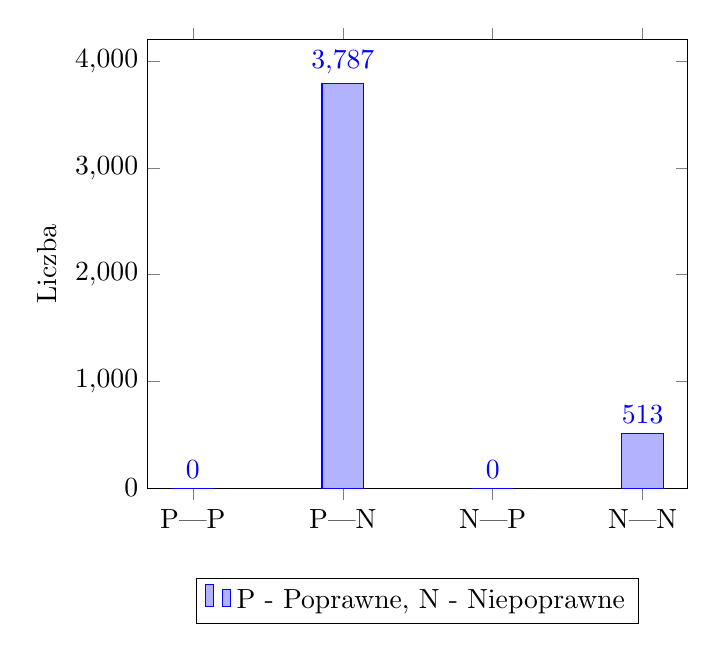
\begin{tikzpicture}
\begin{axis}[
    ybar,
    symbolic x coords={P|P, P|N, N|P, N|N},
    xtick=data,
    ylabel={Liczba},
    nodes near coords,
    bar width=15pt,
    legend style={at={(0.5,-0.20)}, anchor=north, legend columns=-1},
    ymin=0,
    ymax=4200,
]
\addplot coordinates {(P|P,0) (P|N,3787) (N|P,0) (N|N,513)};
\addlegendentry{P - Poprawne, N - Niepoprawne}
\end{axis}
\end{tikzpicture}
\caption{Wykres wyników sprawdzenia poprawności dla zbioru testowego przy zastosowaniu kontrolnego DMJ oraz generatora kodu.}\label{rys:plama2k}
\end{figure}

Dla lepszej wizualizacji wyników zestawiono liczbowo wartości modeli sklasyfikowanych jako \textbf{poprawne} dla generatora \akronim{ZIMPL} oraz kontrolnego DMJ. %Wartość \( z \) przedstawiona w~Tabeli~\ref{tab:experiment:analysis4} wynosi -82,26 zatem różnica jest statystycznie istotna.
Test Z na różnice proporcji na poziomie istotności $\alpha=0,05$ zwraca $p$-wartość $\approx 0$, a więc różnica na korzyść generatora jest istotna.

\begin{table}[H]
\caption{Estymacja przedziału ufności wraz z testem Z na różnice proporcji.}\label{tab:experiment:analysis4}
\centering%
\begin{tabular}{|l|c|c|}
\hline
\textbf{Kategoria} & \textbf{Generator} & \textbf{Kontrolny DMJ} \\
\hline
\textbf{Liczba modeli ($n$)} & 4300 & 4300 \\
\hline
\textbf{Poprawne modele ($m$)} & 3787 & 0 \\
\hline
\textbf{Proporcja (\%)} & 88,07 & 0,00 \\
\hline
\textbf{Przedział ufności (95\%)} & [87,10 ; 89,04] & [0,00 ; 0,00] \\
\hline
%\multicolumn{3}{|c|}{Wartość statystyki \( z \): -82,26} \\
\textbf{$p$-wartość testu Z}&\multicolumn{2}{c|}{$<10^{-18}$}\\
\hline
\end{tabular}
\end{table}

\section{Jak dużą poprawę jakości składni uzyskuje generator względem kontrolnego DMJ?}
% TP: TODO: sugeruję zmienić na "Jak dużą poprawę jakości składni uzyskuje generator względem kontrolnego DMJ?" i dalej pisać o kontrolnym DMJ - DONE

Dla modeli PL w formule sztywnej generator uzyskał \textbf{3,31p}, a kontrolny DMJ \textbf{1,81p} na 4\nobreakdash-punktowej skali jakości zdefiniowanej poniżej. Dla modeli PL w formule parametryzowanej, generator uzyskał \textbf{4,75p}, a kontrolny DMJ \textbf{2,78p} na 6-punktowej skali jakości zdefiniowanej poniżej.
% !!! TP: TODO: tutaj wypadałoby zrobić 2 testy statystyczne na różnice generator vs kontrolny DMJ; ta skala punktowa jest arbitralna, więc rozkład wartości może być nietypowy i byłbym ostrożny w stosowaniu testów parametrycznych; raczej sugeruję użyć np. Wilcoxona dla alpha=0,05 https://pl.wikipedia.org/wiki/Test_Wilcoxona_dla_par_obserwacji

Dla \textbf{sztywnego formułowania} modeli \textit{ZIMPL} generator uzyskuje poprawę, ale nie jest ona tak wysoka, jak przy parametryzowanych modelach. %Średnio wyniki otrzymują ocenę w 3,31, podczas gdy dla kontrolnego DMJ ten wynik zmniejsza się o 1,50 punktu (średnio 1,81). Do testów statystycznych z
Zastosowano test Wilcoxona dla par obserwacji na poziomie istotności $\alpha=0,05$ dla oceny różnic w ocenach uzyskując p-wartość \( 3{,}40 \times 10^{-260} \). Można zatem stwierdzić, że różnica między wynikami jest \textbf{istotna statystycznie}.

\begin{table}[H]
\caption{Tabela sumarycznej oceny wyników dla kodowanych sztywno modeli.}\label{tab:tabela16}
\centering%
\begin{tabular}{|l|c|c|}
\hline
\textbf{Punktacja} & \textbf{Generator} & \textbf{Kontrolny DMJ}\\
\hline
0 & 103 & 509 \\
\hline
1 & 46 & 442 \\
\hline
2 & 386 & 298 \\
\hline
3 & 259 & 1026 \\
\hline
4 & 1481 & 0 \\
\hline
\textbf{Średnia ocena} & \textbf{3,31} & \textbf{1,81} \\
%\hline
%\multicolumn{3}{|c|}{Statystyka testu: \(145788,5\)} \\
\hline
$p$-wartość&\multicolumn{2}{|c|}{\(3{,}40 \times 10^{-260} \)} \\
\hline
\end{tabular}
\end{table}

\begin{figure}[H]
\centering
\begin{minipage}{0.45\textwidth}
\centering
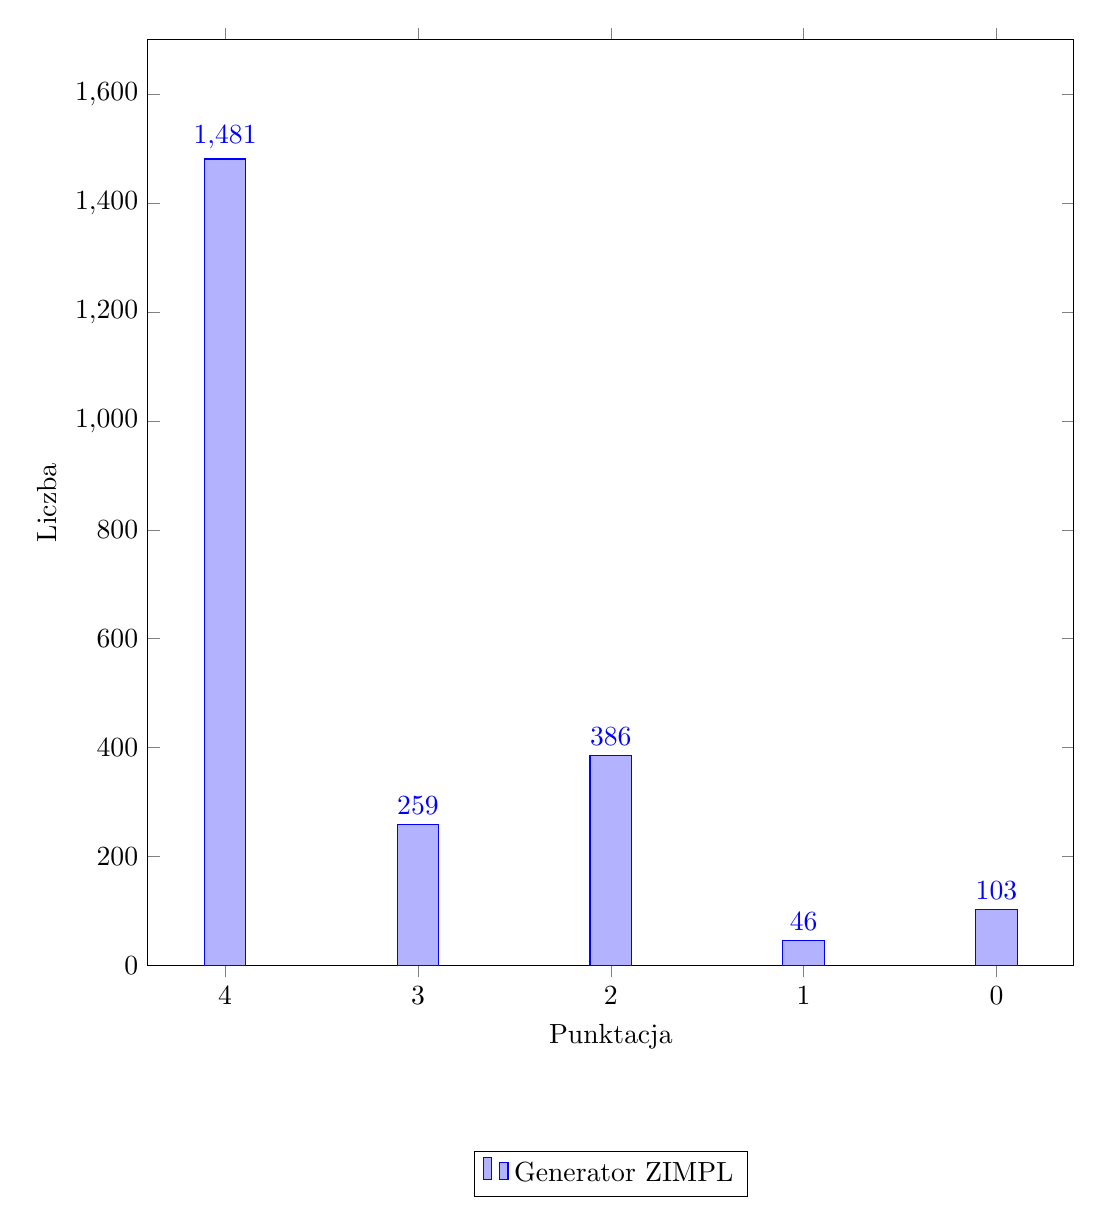
\begin{tikzpicture}
\begin{axis}[
    ybar,
    symbolic x coords={4,3,2,1,0},
    xtick=data,
    ylabel={Liczba},
    width=1.1\textwidth,
    height=1.1\textwidth,
    nodes near coords,
    bar width=15pt,
    ymin=0,
    ymax=1700,
    xlabel={Punktacja},
    legend style={at={(0.5,-0.20)}, anchor=north, legend columns=-1}
]
\addplot coordinates {(4,1481) (3,259) (2,386) (1,46) (0,103)};
\addlegendentry{Generator ZIMPL}
\end{axis}
\end{tikzpicture}
\end{minipage}%
\hspace{0.05\textwidth}
\begin{minipage}{0.45\textwidth}
\centering
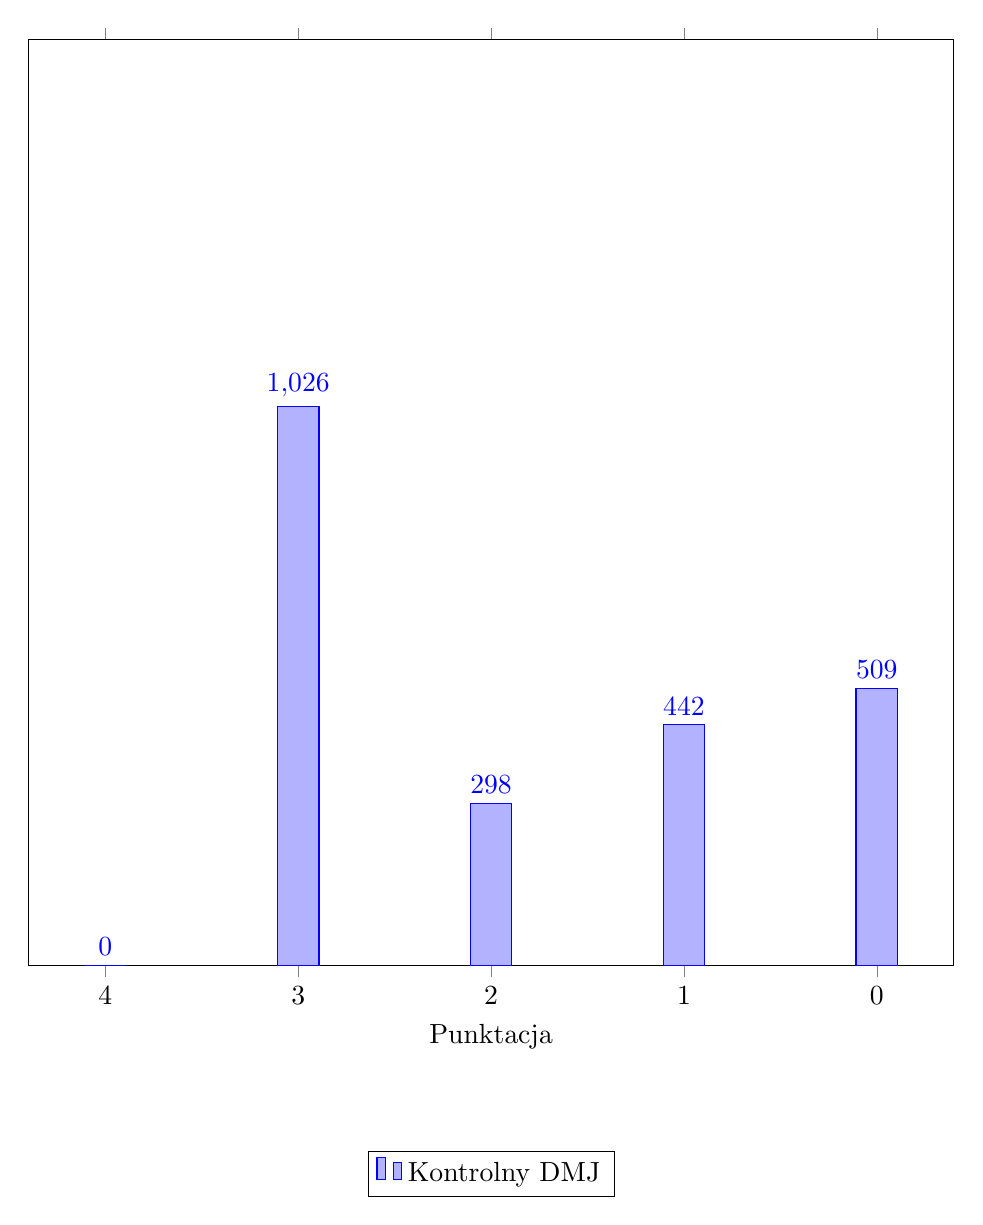
\begin{tikzpicture}
\begin{axis}[
    ybar,
    symbolic x coords={4,3,2,1,0},
    xtick=data,
    %ylabel={Liczba},
    width=1.1\textwidth,
    height=1.1\textwidth,
    ytick = \empty,
    nodes near coords,
    bar width=15pt,
    ymin=0,
    ymax=1700,
    xlabel={Punktacja},
    legend style={at={(0.5,-0.20)}, anchor=north, legend columns=-1}
]
\addplot coordinates {(4,0) (3,1026) (2,298) (1,442) (0,509)};
\addlegendentry{Kontrolny DMJ}
\end{axis}
\end{tikzpicture}
\end{minipage}
\caption{Wykres prezentujący sumaryczną ocenę wyników dla parametryzowanych modeli.} % TP: TODO: ...dla modeli w sztywnej formule?
\end{figure}

W przypadku zestawienia wyników dla modeli parametryzowanych widać, że stworzony generator kodu \textit{ZIMPL} ponownie został lepiej oceniony niż kontrolny DMJ. W~większości wypadków utrzymuje on wynik w okolicy 5 punktów (średnio 4,75). Ta różnica jest znacząca w porównaniu do wyniku kontrolnego DMJ, który jest niższy o 1,97 punktu utrzymując średni poziom 2,78 punktu. Do testów statystycznych ponownie zastosowano test Wilcoxona dla par obserwacji na poziomie istotności $\alpha=0,05$ uzyskując $p$-wartość \textbf{\( 3{,}37 \times 10^{-285} \)}. %Jest to znacznie mniejsza wartość od typowego poziomu istotności. 
Można stwierdzić, że różnica między wynikami jest \textbf{istotna statystycznie}.

\begin{table}[H]
\caption{Tabela sumarycznej oceny wyników dla parametryzowanych modeli.}\label{tab:tabela23}
\centering%
\begin{tabular}{|l|c|c|}
\hline
\textbf{Punktacja} & \textbf{Generator} & \textbf{Kontrolny DMJ}\\
\hline
0 & 3 & 3 \\
\hline
1 & 1 & 80 \\
\hline
2 & 23 & 464 \\
\hline
3 & 293 & 650 \\
\hline
4 & 61 & 789 \\
\hline
5 & 1080 & 39 \\
\hline
6 & 564 & 0 \\
\hline
\textbf{Średnia ocena} & \textbf{4,75} & \textbf{2,78} \\
%\hline
%\multicolumn{3}{|c|}{Statystyka testu: \(45382,0\)} \\
\hline
$p$-wartość&\multicolumn{2}{|c|}{\(3{,}37 \times 10^{-285} \)} \\
\hline
\end{tabular}
\end{table}

\begin{figure}[H]
\centering
\begin{minipage}{0.45\textwidth}
\centering
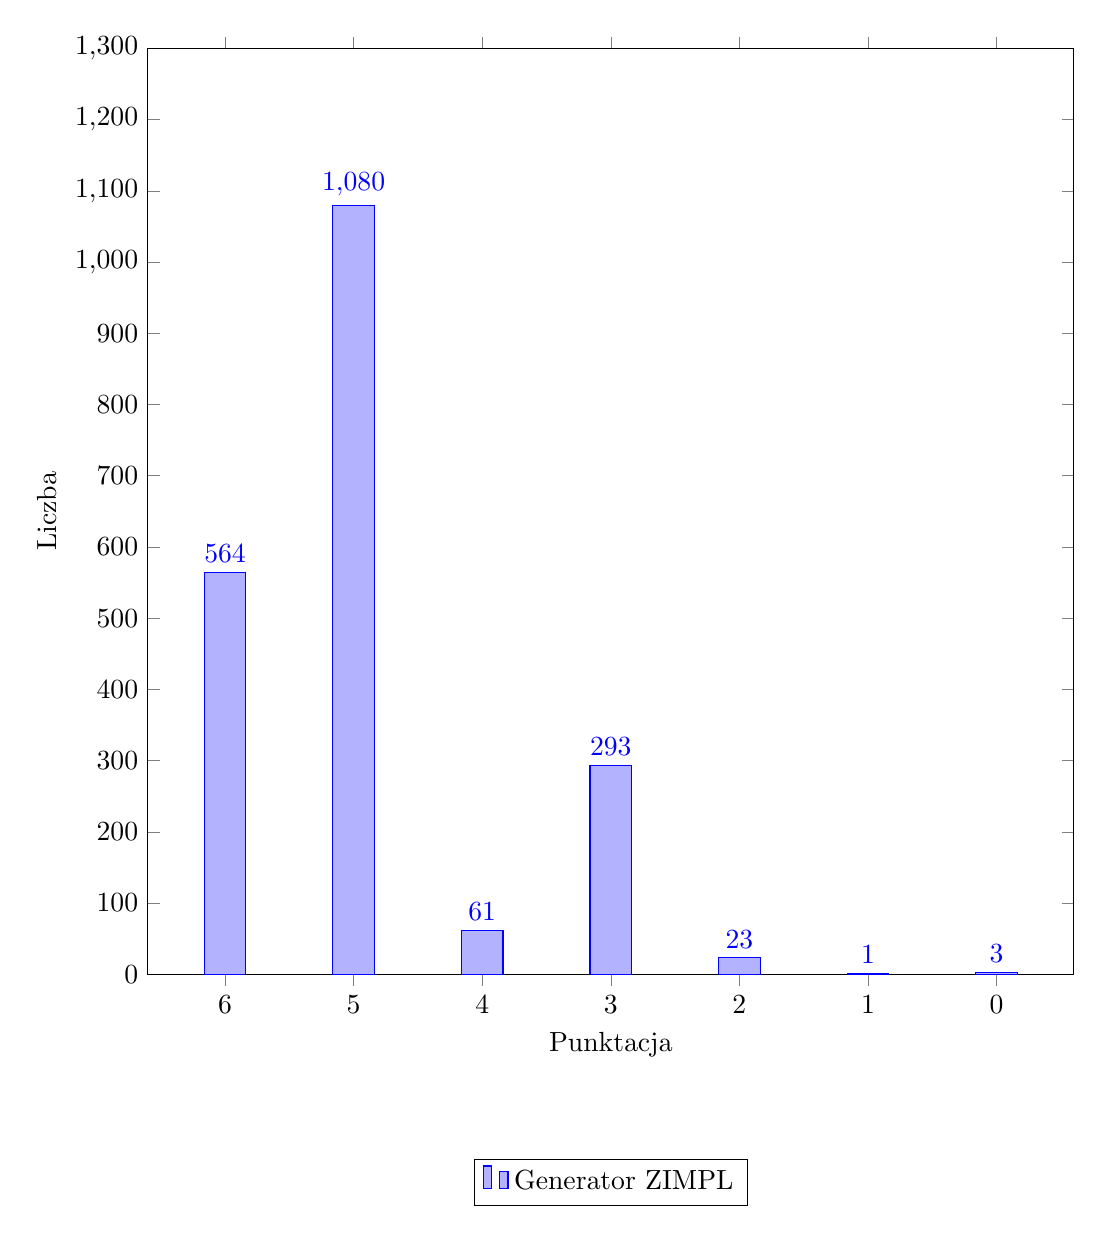
\begin{tikzpicture}
\begin{axis}[
    ybar,
    symbolic x coords={6,5,4,3,2,1,0},
    xtick=data,
    ylabel={Liczba},
    width=1.1\textwidth,
    height=1.1\textwidth,
    nodes near coords,
    bar width=15pt,
    ymin=0,
    ymax=1300,
    xlabel={Punktacja},
    legend style={at={(0.5,-0.20)}, anchor=north, legend columns=-1}
]
\addplot coordinates {(6,564) (5,1080) (4,61) (3,293) (2,23) (1,1) (0,3)};
\addlegendentry{Generator ZIMPL}
\end{axis}
\end{tikzpicture}
\end{minipage}%
\hspace{0.05\textwidth}
\begin{minipage}{0.45\textwidth}
\centering
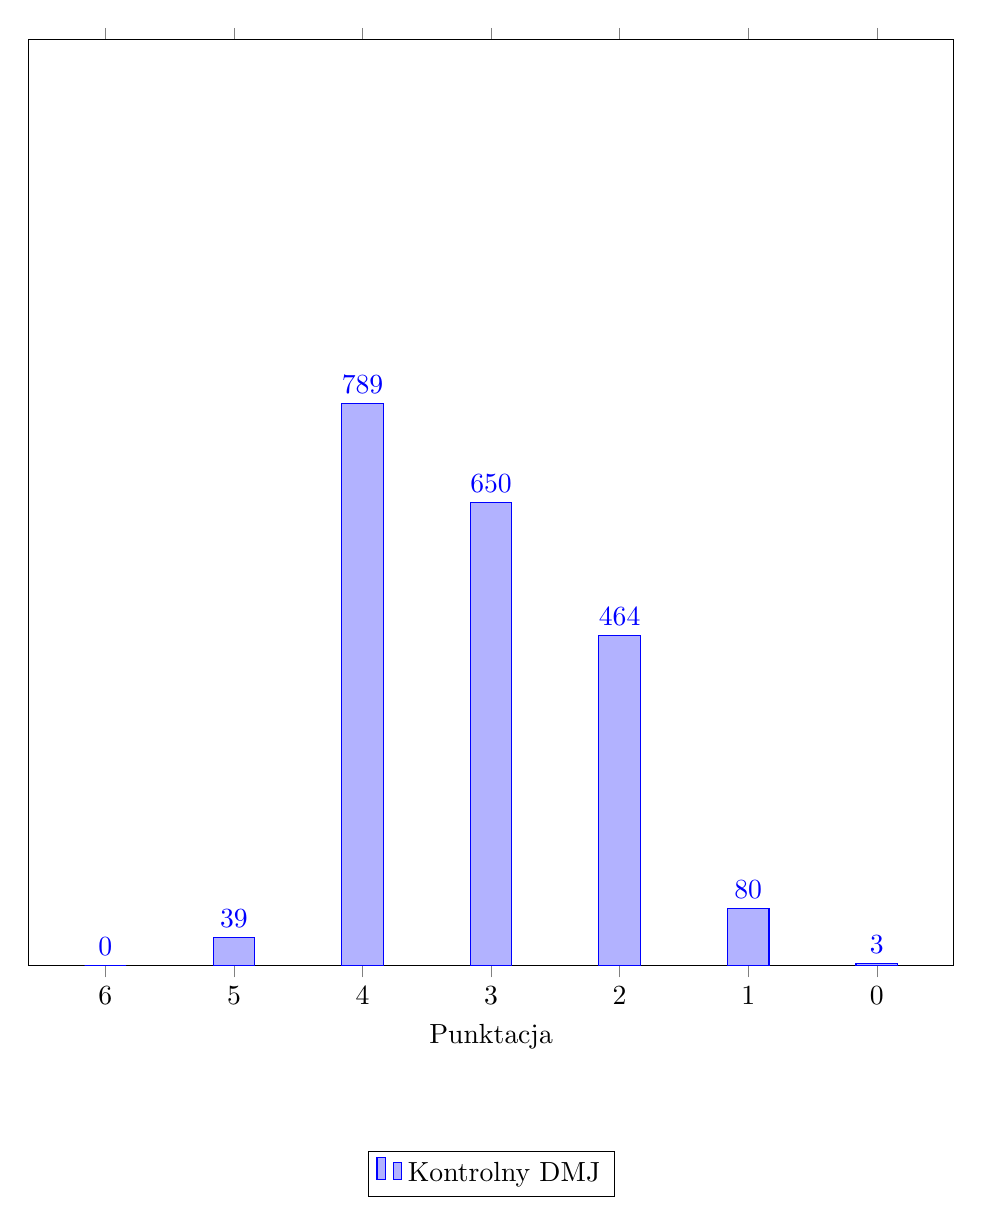
\begin{tikzpicture}
\begin{axis}[
    ybar,
    symbolic x coords={6,5,4,3,2,1,0},
    xtick=data,
    %ylabel={Liczba},
    width=1.1\textwidth,
    height=1.1\textwidth,
    ytick = \empty,
    nodes near coords,
    bar width=15pt,
    ymin=0,
    ymax=1300,
    xlabel={Punktacja},
    legend style={at={(0.5,-0.20)}, anchor=north, legend columns=-1}
]
\addplot coordinates {(6,0) (5,39) (4,789) (3,650) (2,464) (1,80) (0,3)};
\addlegendentry{Kontrolny DMJ}
\end{axis}
\end{tikzpicture}
\end{minipage}
\caption{Wykres prezentujący sumaryczną ocenę wyników dla parametryzowanych modeli.}
\end{figure}



Do sprawdzenia jakości modelu PL pod względem jego składni i jakości zrozumienia zadania zastosowano ocenę ekspercką, w~której ekspert przyznawał punkty dla czterech (formuła sztywna) lub sześciu (formuła parametryzowana) kryteriów. W~roli eksperta wykorzystano DMJ \textit{GPT-4o}, który jest niezależny od DMJ stosowanych w generatorze i kontrolnym DMJ. Po otrzymaniu wyników, dla większej wiarygodności, wykonano oczyszczanie rezultatów i naprawę oczywistych błędów halucynowanych przez DMJ. % TP: TODO <- opiszcie dokładnie procedurę czyszczenia i naprawy; jak dobrze rozumiem, w Sekcji 5.4 nie było takiej procedury; gdyby jednak była też tam stosowana, to wtedy możecie to czyszczenie dodać do opisu kontrolengo DMJ z sekcji 5.1

Tak jak w przypadku generowania, zastosowano wartość temperatury równą 0 oraz maksymalną liczbę tokenów równą 512. Dokładna procedura uruchomienia DMJ i oczyszczania odpowiedzi wyglądała następująco:

\begin{enumerate}
\item Do skryptu w języku \akronim{Python} wprowadzano poprawny model PL, model stworzony przez generator \akronim{ZIMPL}, model stworzony przez kontrolny DMJ oraz wartość 1, jeżeli kod był parametryzowany lub 0, jeżeli kod był w sztywnej formule.
\item Zależnie od wprowadzonej wartości uruchamiany był DMJ wraz z odpowiednim zapytaniem. DMJ dla pojedynczego problemu PL uruchamiany był dwukrotnie, tak aby zweryfikować i~nadać punktację dla modelu generatora oraz modelu kontrolnego DMJ.

Zapytania do oceny posiadają podobny schemat. Różnią się jedynie ilością kryteriów oceny. Schemat zapytania wygląda następująco:

\begin{lstlisting}[language=zimpl]
<Określenie celu zapytania>
<Określenie kryteriów zapytania i sposobu interpretacji wyników oraz liczby nadawanych
punktów>
<Schemat odpowiedzi w formie kategoria: punkty; wyjaśnienie>
<Przykładowy rezultat działania zapytania>
\end{lstlisting}

Dokładny przebieg analizy wyglądał następująco:

\begin{enumerate}
\item \textbf{Zapytanie dla wartości 0} --- sprawdzało podany kod względem poprawnego kodu PL i~oceniało go w~4.~kategoriach szczegółowo opisanych w~Rozdziale~\ref{ch:experiment:hardcoded}.
\item \textbf{Zapytanie dla wartości 1} --- sprawdzało podany kod względem poprawnego kodu PL i~oceniało go w~6.~kategoriach szczegółowo opisanych w~Rozdziale~\ref{ch:experiment:parameters}.
\end{enumerate}
\item Otrzymane wyniki zapisane zostały w arkuszu kalkulacyjnym, gdzie po analizie odpowiedzi dokonano oczyszczenia rezultatów z~widocznych błędów, których nie dało się wykluczyć w procesie tworzenia zapytań.
\begin{enumerate}
\item Zmieniono punktacje na 0 dla wszystkich modeli, które przy tworzeniu ograniczeń zastosowały nazwę \textit{s.t.} lub \textit{subject}, zamiast \textit{subto}.
\item Zmieniono punktacje na 1 dla wszystkich modeli, które posiadały komentarz o braku problemów w~kategorii innych wymagań, jak brak zbędnych poleceń, poprawne rozpoczęcie linii od kluczowych słów oraz poprawne użycie prefiksu \textit{\#} komentarzy, a~w~wyniku halucynacji modelu otrzymały 0~punktów.
\item Zmieniono punktację na 1 dla wszystkich modeli, dla których w kategorii innych wymagań niesłusznie dano 0~punktów za stawianie średników na końcu wierszy kodu.
\end{enumerate}
\end{enumerate}

% TP: TODO: tutaj brakuje też dokładnego udokumentowania procedury odpytania DMJ, tzn. jakiego prompta dostał? Czy to była sekwencja pytań i odpowiedzi? itd. Jako, że prompty są pewnie dedykowane pod formułę poniżej, to możecie je pokazać w poniższych sekcjach. - DONE

%Zależnie od funkcjonalności kodu, wykorzystano inne mierniki jakości. Dla wyników parametryzowanych zastosowano skalę sześciostopniową, podczas gdy dla sztywnego kodowania - czterostopniową.

%Wynikiem eksperymentu jest punktacja \textbf{3,31/4,00} dla wygenerowanych wyników, w porównaniu do \textbf{1,81/4,00} dla standardowego zapytania, dla wszystkich wyników sztywnego kodowania. Tak samo, dla parametryzowanych wyników powstałych w wyniku wykorzystania generatora oceną jest \textbf{4,75/6,00}, podczas gdy dla pojedynczego zapytania wynosi \textbf{2,78/6,00}. Sumaryczna poprawa względem standardowego zapytania \textbf{wzrosła o średnio 1,74} punktu.

\subsection{Modele PL w sztywnej formule.}\label{ch:experiment:hardcoded}

Dla wynikowych modeli PL w \textbf{sztywnej formule} poddano ocenie poniższe kryteria binarne w odniesieniu do wzorcowego modelu PL zawartego w danych testowych. Kryteria oceniano, przyznając $1$ lub $0$ punktów. Nie stosowano punktów połówkowych.

\begin{enumerate}
\item \textbf{Definiowanie zmiennych} -- $1$p jeśli \textbf{wszystkie} zmienne i ich typy są zgodne z modelem wzorcowym. Nazwy zmiennych i komentarze mogą się różnić, ale logika ich wykorzystania musi pozostać taka sama. Dowolne niespełnienie tego wymagania powoduje przyznanie $0$p.
\item \textbf{Funkcja celu} -- $1$p jeśli funkcja celu jest semantycznie równa funkcji celu w modelu wzorcowym, łącznie z~kierunkiem optymalizacji. Semantyczna równość to równość algebraiczną po uzgodneniu mapowania między nazwami zmiennych w obu modelach. Nazwy funkcji i~zmiennych nie mają znaczenia. Funkcje niezgodne semantycznie skutkują przyznaniem $0$p.
\item \textbf{Ograniczenia} -- aby otrzymać $1$p, ograniczenia muszą być zdefiniowane zgodnie ze wzorcowym modelem. Liczba, logika i zapis muszą być zgodne, a każde ograniczenie powinno zaczynać się od \texttt{subto <nazwa>:}. Zastosowanie innej struktury powoduje przyznanie $0$p.
\item \textbf{Inne wymagania} -- $1$p przyznaje się za spełnienie wymagań takich jak: użycie \texttt{\#} jako prefiksu komentarzy, brak zbędnych poleceń (\texttt{solve}, \texttt{subject to}) oraz poprawne rozpoczęcie każdej linii od jednego z kluczowych słów (\texttt{var}, \texttt{minimize}, \texttt{maximize}, \texttt{subto}).
\end{enumerate}

Poniżej przedstawiona została analiza wyników generatora oraz kontrolnego DMJ dla poszczególnych kategorii.

\begin{table}[H]
\caption{Tabela ocenionych wyników dla kategorii \textbf{Definiowanie zmiennych}.}\label{tab:tabela12}
\centering%
\begin{tabular}{|l|c|c|}
\hline
\textbf{Punktacja} & \textbf{Generator} & \textbf{Kontrolny DMJ}\\
\hline
1 & 1832 & 1418 \\
\hline
0 & 443 & 857 \\
\hline
Średnia ocena & 0,81 & 0,62 \\
\hline
%\multicolumn{3}{|c|}{Wartość statystyki \( z-score \): 13,59} \\
$p$-wartość testu Z&\multicolumn{2}{c|}{$<10^{-18}$}\\
\hline
\end{tabular}
\end{table}

% TP: !!! test statystyczny na różnice średnich/frakcje dla \alpha=0,05, np. https://pl.wikipedia.org/wiki/Test_dla_proporcji#Test_dla_dwóch_prób_dużych - DONE

Już pierwszy wynik pokazuje większą skuteczność generatora ponad kontrolnym DMJ. Podstawowym błędem popełnianym w deklaracji zmiennych jest niezgodna w porównaniu z zadaniem ich liczba. Problem posiadają oba DMJ, natomiast kontrolny DMJ zmaga się również częściowo z błędną deklaracją zmiennych. Dla testu Z na różnice średnich na poziomie istotności $\alpha = 0,05$, %z-score wynosi \textbf{13,59}
$p$-wartość wynosi $\approx 0$. W~związku z~tym różnica między proporcjami wyników \textbf{jest istotna}.

% TP: za dużo? za mało? nieadekwatne zmienne? Macie na to jakieś statystyki do pokazania? - DONE

\begin{table}[H]
\caption{Tabela ocenionych wyników dla kategorii \textbf{Funkcja celu}.}\label{tab:tabela13}
\centering%
\begin{tabular}{|l|c|c|}
\hline
\textbf{Punktacja} & \textbf{Generator} & \textbf{Kontrolny DMJ}\\
\hline
1 & 1882 & 1469 \\
\hline
0 & 393 & 806 \\
\hline
Średnia ocena & 0,83 & 0,65 \\
\hline
%\multicolumn{3}{|c|}{Wartość statystyki \( z-score \): 13,90} \\
$p$-wartość testu Z&\multicolumn{2}{c|}{$<10^{-18}$}\\
\hline
\end{tabular}
\end{table}

% TP: TODO: test statystyczny jw.

Generator tworzy poprawne funkcje celu częściej od kontrolnego DMJ. 
Znacznie większe różnice zachodzą dla ograniczeń. Kontrolny DMJ w każdym z przypadków testowych generuje kod zawierający w sobie niepoprawną deklarację ograniczenia, przez co nigdy nie został sklasyfikowany jako poprawny. Dla testu Z na różnice średnich dla $\alpha = 0,05$, %z-score wynosi \textbf{13,90}, zatem zwiększył się w stosunku do poprzedniego przykładu
$p$-wartość wynosi $\approx0$. Różnica między proporcjami wyników \textbf{jest istotna}.
% TP: w tabeli jednak widać, że zdobywa jedyniki - chyba błąd w danych; zobaczcie, że średnie też nie pasują do danych. - done, poprawione

\begin{table}[H]
\caption{Tabela ocenionych wyników dla kategorii \textbf{Ograniczenia}.}\label{tab:tabela14}
\centering%
\begin{tabular}{|l|c|c|}
\hline
\textbf{Punktacja} & \textbf{Generator} & \textbf{Kontrolny DMJ}\\
\hline
1 & 2140 & 0 \\
\hline
0 & 135 & 2275 \\
\hline
Średnia ocena & 0,94 & 0,00 \\
\hline
%\multicolumn{3}{|c|}{Wartość statystyki \( z-score \): 63,56} \\
$p$-wartość testu Z&\multicolumn{2}{c|}{$<10^{-18}$}\\
\hline
\end{tabular}
\end{table}

% TP: TODO: test statystyczy jw.

Największą trudnością kontrolnego DMJ jest uzyskanie pozytywnej punktacji w kategorii \textbf{Ograniczenia}. Dzieje się tak przez niepoprawny zapis początku linii deklarującej ograniczenie. W związku z tymi problemami, test Z na różnice średnich dla $\alpha = 0,05$, %wykazał z-score równe \textbf{63,56}, znacząco odstając od wcześniejszych wyników
$p$-wartość $\approx0$. Różnica między proporcjami wyników \textbf{jest istotna}.

\begin{table}[H]
\caption{Tabela ocenionych wyników dla kategorii \textbf{Inne wymagania}.}\label{tab:tabela15}
\centering%
\begin{tabular}{|l|c|c|}
\hline
\textbf{Punktacja} & \textbf{Generator} & \textbf{Kontrolny DMJ}\\
\hline
1 & 1665 & 1229 \\
\hline
0 & 610 & 1046 \\
\hline
Średnia ocena & 0,73 & 0,54 \\
\hline
%\multicolumn{3}{|c|}{Wartość statystyki \( z-score \): 13,43} \\
$p$-wartość testu Z&\multicolumn{2}{c|}{$<10^{-18}$}\\
\hline
\end{tabular}
\end{table}

% TP: test statystyczny - DONE

Kategoria \textbf{Inne wymagania} zwraca rezultaty zbliżone do pierwszych dwóch kategorii. Dla testu Z na różnice średnich dla $\alpha = 0,05$, %wykazał z-score równe \textbf{13,43}, co jest najniższym z dotychczasowych wyników
$p$-wartość wynosi $\approx0$. Różnica między proporcjami wyników \textbf{jest istotna}.

\subsection{Modele PL w parametryzowanej formule.}\label{ch:experiment:parameters}

Dla wynikowych modeli PL w \textbf{formule parametryzowanej} poddano ocenie poniższe kryteria binarne w~odniesieniu do wzorcowych modeli PL zawartych w danych testowych. Kryteria oceniano przyznając $1$ lub $0$ punktów. Nie stosowano punktów połówkowych. Punktacja w tym przypadku wygląda następująco:
%Podobna analiza została przeprowadzona dla modeli parametryzowanych. Dla kategorii, jakie przedstawiają, przewaga generatora jest znacznie wyższa. Wynika to z złożoności kodu, z jakim pracuje. Modele generowane za pomocą pojedynczego zapytania nie posiadają wiedzy na temat struktury kodu, przez co mają problemy z identyfikacją zbiorów i parametrów. Punktacja w tym przypadku jest w kategoriach:

\begin{enumerate}
\item \textbf{Definiowanie zbiorów} -- $1$p jeśli wszystkie zbiory są poprawnie zdefiniowane przy użyciu nawiasów klamrowych \texttt{\{\}}, z elementami w cudzysłowach. Nazwy zmiennych i~komentarze mogą się różnić, ale logika ich wykorzystania musi pozostać taka sama. Dowolne niespełnienie tego wymagania powoduje przyznanie $0$p. % TP: TODO: a jeśli wartościami zbioru są liczby? - w naszych zbiorach nadal są definiowane zgodnie z tym schematem
\item \textbf{Definiowanie parametrów} -- $1$p jeśli wszystkie parametry są poprawnie zindeksowane za pomocą nawiasów kwadratowych \texttt{[ ]}, schematu \texttt{<klucz> wartość} lub tablicy i logicznie zgodne z celem zadania. Nazwy parametrów mogą się różnić, o~ile zachowano ich poprawne zastosowanie. Każde odstępstwo od reguły skutkuje przyznaniem $0$ punktów.
\item \textbf{Definiowanie zmiennych} -- $1$p jeśli wszystkie zmienne i~ich dziedziny są zgodne z~modelem wzorcowym. Zmienne muszą być indeksowane odpowiednimi zbiorami. Nazwy zmiennych i~komentarze mogą się od różnić, ale logika ich wykorzystania musi pozostać taka sama. Brak zgodności powoduje przyznanie $0$p.
\item \textbf{Funkcja celu} -- $1$p jeśli funkcja celu jest semantycznie równa funkcji celu w~modelu wzorcowym, łącznie z~kierunkiem optymalizacji. Semantyczna równość to równość algebraiczną po uzgodnieniu mapowania między nazwami zmiennych w~obu modelach. Nazwy funkcji i~zmiennych nie mają znaczenia. Funkcje niezgodne semantycznie skutkują przyznaniem $0$p.
\item \textbf{Ograniczenia} -- aby otrzymać $1$p, ograniczenia muszą być zdefiniowane zgodnie ze wzorcowym modelem. Liczba, logika i zapis muszą być zgodne, a~każde ograniczenie powinno zaczynać się od \texttt{subto <nazwa>:}. Zastosowanie innej struktury powoduje przyznanie $0$p.
\item \textbf{Inne wymagania} -- $1$p przyznaje się za spełnienie wymagań takich jak: użycie \texttt{\#} jako prefiksu komentarzy, brak zbędnych poleceń oraz poprawne rozpoczęcie każdej linii od jednego ze słów kluczowych (\texttt{var}, \texttt{minimize}, \texttt{maximize}, \texttt{subto}). 
\end{enumerate}

% TP: TODO: poprawcie proszę niżej analogicznie do sekcji 5.5.1 -> ja kontynuuję sprawdzanie w Rozdziale 6

Już w pierwszej kategorii przedstawionej w tabeli~\ref{tab:tabela17} widać znaczącą różnicę w wynikach między generowanymi wynikami. Kontrolny DMJ nie radzi sobie z tworzeniem zbiorów, stosując błędną implementację. Średnie wyniki uzyskanej punktacji różnią się od siebie o \textbf{0,33} punktu. Dla testu Z na różnice średnich dla $\alpha = 0,05$, %, wykazał z-score równe \textbf{28,95}
$p$-wartość wynosi $\approx0$. W związku z tym wynikiem, można stwierdzić, że różnica między proporcjami wyników \textbf{jest istotna}.

\begin{table}[H]
\caption{Tabela ocenionych wyników dla kategorii \textbf{Definiowanie zbiorów}.}\label{tab:tabela17}
\centering%
\begin{tabular}{|l|c|c|}
\hline
\textbf{Punktacja} & \textbf{Generator} & \textbf{Kontrolny DMJ}\\
\hline
1 & 1783 & 914 \\
\hline
0 & 242 & 1111 \\
\hline
Średnia ocena & 0,88 & 0,45 \\
\hline
%\multicolumn{3}{|c|}{Wartość statystyki \( z-score \): 28,95} \\
$p$-wartość testu Z&\multicolumn{2}{c|}{$<10^{-18}$}\\
\hline
\end{tabular}
\end{table}

Tabela~\ref{tab:tabela18} prezentuje rozkład punktów przyznanych za definiowanie parametrów. Opracowany generator uzyskuje około 99\% skuteczności. Wyniki kontrolnego DMJ również utrzymują się na poziomie powyżej 80\%. %Mimo tego z-score jest równy \textbf{18,61}, co w dalszym ciągu pokazuje, że
Test Z na różnice średnich dla $\alpha=0,05$ zwraca $p$-wartość $\approx0$, stąd 
różnica między proporcjami wyników \textbf{jest istotna}.

\begin{table}[H]
\caption{Tabela ocenionych wyników dla kategorii \textbf{Definiowanie parametrów}.}\label{tab:tabela18}
\centering%
\begin{tabular}{|l|c|c|}
\hline
\textbf{Punktacja} & \textbf{Generator} & \textbf{Kontrolny DMJ}\\
\hline
1 & 2008 & 1663 \\
\hline
0 & 17 & 362 \\
\hline
Średnia ocena & 0,99 & 0,82 \\
\hline
%\multicolumn{3}{|c|}{Wartość statystyki \( z-score \): 28,95} \\
$p$-wartość testu Z&\multicolumn{2}{c|}{$<10^{-18}$}\\
\hline
\end{tabular}
\end{table}

Definiowanie zmiennych na podstawie zbiorów i parametrów obniża jakość wyniku kodu, przez co nie zostaje osiągnięta 100\% poprawność, tak jak w przypadku sztywnego formatu kodu. Tabela~\ref{tab:tabela19} przedstawia %\textbf{z}, którego wartość wynosi \textbf{9,20}
$p$-wartość $\approx0$, co w dalszym ciągu wskazuje, że różnica między proporcjami wyników \textbf{jest istotna}.

\begin{table}[H]
\caption{Tabela ocenionych wyników dla kategorii \textbf{Definiowanie zmiennnych}.}\label{tab:tabela19}
\centering%
\begin{tabular}{|l|c|c|}
\hline
\textbf{Punktacja} & \textbf{Generator} & \textbf{Kontrolny DMJ}\\
\hline
1 & 1713 & 1473 \\
\hline
0 & 312 & 552 \\
\hline
Średnia ocena & 0,85 & 0,73 \\
\hline
%\multicolumn{3}{|c|}{Wartość statystyki \( z-score \): 9,20} \\
$p$-wartość testu Z&\multicolumn{2}{c|}{$<10^{-18}$}\\
\hline
\end{tabular}
\end{table}


W przypadku definiowania funkcji celu, wyniki obu modeli są zbliżone do siebie. Poza wynikiem procentowym równym 99\%, %jako jedyna kategoria, posiada \textit{z} = \textbf{0,29}, które mieści się w zakresie
$p$-wartość testu Z na różnice średnich na poziomie istotności $\alpha=0,05$ wynosi $0,772$
 i wskazuje, że różnica między proporcjami wyników \textbf{nie jest istotna}.

\begin{table}[H]
\caption{Tabela ocenionych wyników dla kategorii \textbf{Funkcja celu}.}\label{tab:tabela20}
\centering%
\begin{tabular}{|l|c|c|}
\hline
\textbf{Punktacja} & \textbf{Generator} & \textbf{Kontrolny DMJ}\\
\hline
1 & 2002 & 2000 \\
\hline
0 & 23 & 25 \\
\hline
Średnia ocena & 0,99 & 0,99 \\
\hline
%\multicolumn{3}{|c|}{Wartość statystyki \( z-score \): 0,29} \\
$p$-wartość testu Z&\multicolumn{2}{c|}{$0,772$}\\
\hline
\end{tabular}
\end{table}

Znacząca różnica pojawia się przy porównywaniu ograniczeń. Kontrolny DMJ nie zna składni kodu  \textit{ZIMPL}, w związku z czym każdorazowo deklaruje niepoprawne ograniczenia, używając takich elementów jak \texttt{s.t.} lub \texttt{subject to}. %\textit{z-score} jest równy \textbf{56,64}
$p$-wartość testu Z wynosi $\approx0$, zatem różnica między proporcjami wyników \textbf{jest istotna}.

\begin{table}[H]
\caption{Tabela ocenionych wyników dla kategorii \textbf{Ograniczenia}.}\label{tab:tabela21}
\centering%
\begin{tabular}{|l|c|c|}
\hline
\textbf{Punktacja} & \textbf{Generator} & \textbf{Kontrolny DMJ}\\
\hline
1 & 1790 & 0 \\
\hline
0 & 235 & 2025 \\
\hline
Średnia ocena & 0,88 & 0,00 \\
\hline
%\multicolumn{3}{|c|}{Wartość statystyki \( z-score \): 56,64} \\
$p$-wartość testu Z&\multicolumn{2}{c|}{$<10^{-18}$}\\
\hline
\end{tabular}
\end{table}


W przypadku oceny innych wymagań w Tabeli~\ref{tab:tabela22}, oba DMJ osiągnęły niskie oceny. Wynikało to ponownie z ogólności kategorii. Wszelkie błędy, które nie zostały wyłapane w pozostałych kategoriach, zostały rozliczone w tym miejscu. Wygenerowane modele straciły najwięcej punktów na wykorzystywaniu niepotrzebnych i niezwiązanych z problemem komend. Dla testu Z na różnice średnich dla $\alpha = 0,05$, %, wykazał z-score równe \textbf{14,98}. 
$p$-wartość wynosi $\approx0$.
W związku z tym wynikiem, można stwierdzić, że różnica między proporcjami wyników \textbf{jest istotna}.

\begin{table}[H]
\caption{Tabela ocenionych wyników dla kategorii \textbf{Inne wymagania}.}\label{tab:tabela22}
\centering%
\begin{tabular}{|l|c|c|}
\hline
\textbf{Punktacja} & \textbf{Generator} & \textbf{Kontrolny DMJ}\\
\hline
1 & 658 & 259 \\
\hline
0 & 1367 & 1766 \\
\hline
Średnia ocena & 0,32 & 0,13 \\
\hline
%\multicolumn{3}{|c|}{Wartość statystyki \( z-score \): 14,98} \\
$p$-wartość testu Z&\multicolumn{2}{c|}{$<10^{-18}$}\\
\hline
\end{tabular}
\end{table}


\chapter{Dyskusja}

\section{Zalety rozwiązania}

Przedstawione rozwiązanie usprawnia proces generacji modeli \textit{PL}, korzystając z \textit{DMJ} na podstawie opisów słownych. Umożliwia to korzystanie z zalet \textit{PL} dla użytkowników oraz przedsiębiorców, usprawniając tym samym proces optymalizacji rozwiązań. Korzystanie z narzędzia nie wymaga wiedzy eksperckiej z dziedziny optymalizacji. Zaletą tego rozwiązania jest solidne podejście do generacji modeli wykorzystując \textit{DMJ} oraz wiedze ekspercką, zmniejszając tym zauważalnie ilość błędów generowanych przez \textit{DMJ} niekorzystających z powyższych udogodnień. Przekłada się to bezpośrednio na mniejsze koszta uzyskania rozwiązania oraz braku konieczności posiadania wykwalifikowanego personelu w tej dziedzinie. Umożliwia to na rozpowszechnienie ogólnodostępnego rozwiązania w dziedzinie \textit{PL}. 

\section{Wady rozwiązania}
Stworzone narzędzie jest najbardziej wydajne dla prostych instancji problemów \textit{PL} z małą do średniej ilości danych. Przy większej ilości danych \textit{DMJ} może nie działać na satysfakcjonującym poziomie. Wydajność \textit{DMJ} znacząco spada, w miarę wzrostu wielkości kontekstu wejściowego, nawet w przypadku modeli zaprojektowanych do obsługi dużych kontekstów. Rozmiar kontekstu \textit{DMJ}, jest bardzo ograniczony w porównaniu do problemów optymalizacyjnych korzystających z dużej ilości danych wejściowych. \cite{10.1162/tacl_a_00638} Kolejnym ograniczeniem jest zależność pomiędzy jakością generowanego kodu \textit{PL}, a niską różnorodnością dostępnych przykładów w literaturze. Im większa różnorodność dostępnych przykładów w literaturze, tym większa jakość generowanego kodu \textit{PL}.

\section{Poprawa rozwiązania}
Niewątpliwie automatyzacja procesu \textit{uczenia przez wzmacnianie} pozwoliłaby uzyskać bardziej satysfakcjonujące wyniki, pozwalając modelowi dostosować się do bardziej różnorodnych problemów na podstawie nowych oraz wykorzystanych danych. Rozwiązanie zautomatyzowane zostało przedstawione w sekcji \ref{sec:optimus}. 

Zwiększenie ilości oraz różnorodności przykładów również przyczyniłoby się do zwiększenia jakości generowanych modeli \textit{PL}. Jest to rozwiązanie czasochłonne, ponieważ ilość powszechnie dostępnych, profesjonalnych źródeł jest ograniczona.
Hipoteza: Automatyzacja procesu \textit{uczenia przez wzmacnianie} oraz zwiększenie bazy przykładów przyczyniłoby się do poprawy wyników programu.

\section{Trudności}

Początkowo zaczęto tworzyć własny model na jednym z rozwiązań niekomercyjnych metodą \textit{ang. fine-tuningu}. Wydajność tego rozwiązania okazała się niesatysfakcjonująca. Wydajność nie poprawiła się, pomimo zwielokrotnienia bazy przykładów uczących.

Spojrzeć na rozwiązanie wysokopoziomowe, co jest dobre, co jest złe, co można poprawić (postawić hipotezy jak postawić), dlaczego pewnych rzeczy nie da się zrobić (np. duże problemy PL, ograniczenia językowe, etc), odnieść się do innych projektów – co nam nie pomogło, co pomogło, czemu wykorzystaliśmy dane rzeczy

Rozpatrzono użycie różnych \textit{DMJ}, biorąc przy tym pod uwagę najlepszą jakość, przy jak najmniejszym koszcie. Zdecydowaliśmy się na model \texttt{GPT-4o}, odrzucając przy tym modele bardziej wydajne, ze względu na zbyt wysokie koszta obliczeniowe. Skutkiem tej decyzji była konieczność zmiany struktury rozwiązania na bardziej złożoną, co nie jest optymalnym podejściem, gdyż prowadzi do obniżenia przejrzystości oraz zwiększeniu stopniu skomplikowania implementacji.


%Jagoda: Dorzucam do dyskusji, może chcecie gdzieś zawrzeń w ramach wniosków elementy wypowiedzi
Jaki procent modeli stworzonych przez generator ZIMPL
kompiluje się poprawnie?

Test jest istotny, bo pokazuje, że system radzi sobie z formułowaniem możliwych do rozwiązania modeli LP. Zwłaszcza przy modelach LP ze sztywno zapisanym kodem wynikowym, rezultaty pokazują, że generator potrafi w większości wypadków tworzyć prawidłowo składniowe wyniki. % TP: TODO: <- nie jestem przekonany do tego akapitu. W zasadzie powtarza i rozmywa to co zostało powiedziane wczesniej. Takie ogólnikowe stwierdzenia bardziej pasują do dyskusji.

%Jagoda: dorzucam rekomendacje na podstawie wyników eksperymentów:
Na podstawie przeprowadzonych analiz zaleca się dalsze doskonalenie wersji parametryzowanej w celu zwiększenia jej efektywności. Wersja sztywna aktualnie jest rekomendowana jako bardziej niezawodna opcja.

\chapter{Wnioski i dalszy kierunek prac}

\section{Wnioski}
Na początku pracy postawiono hipotezę badawczą:
\begin{quote}
\textit{Można wykorzystać duże modele językowe do generowania modeli PL zapisanych w języku naturalnym.}
\end{quote}

Analizując przedstawione rozwiązanie i wspomagając się eksperymentami założono poprawność powyższej hipotezy. Przy odpowiednio przygotowanym zapytaniu można z dużą pewnością założyć, że duże modele językowe można wykorzystać do generowania modeli PL otrzymując na wejściu jedynie problem zapisany w języku naturalnym. Istnieje znacząca poprawa w jakości wygenerowanego rozwiązania w stosunku do rozwiązania za pomocą pojedynczego, prostego zapytania. Zaobserwowano wzrost skuteczności dużych modeli językowych przy generowaniu modeli \textit{PL}. Przekłada się to na usprawnienie procesu modelowania optymalizacyjnego. 

Wyniki eksperymentu pokazały, iż bardziej precyzyjne oraz szczegółowo sformułowane zapytania, przekładają się bezpośrednio na wzrost jakości wygenerowanego modelu \textit{PL} przez \textit{DMJ}. Redukuje to konieczność kosztownej w zasobach i czasie pracy ekspertów. Rozwiązanie to zmniejsza liczbę błędów oraz redukuje niedoskonałości wykonania wynikające z czynnika ludzkiego. 

Zauważono również, iż zwiększenie różnorodności przykładów przyczyniłoby się do poprawy jakości generowanych modeli \textit{PL} przez duże modele językowe. Tworzy to dodatkowe adaptacje dla dużych modeli językowych oraz polepsza ich elastyczność.

\section{Dalszy kierunek prac}

Kolejnym etapem rozwoju sytemu generującego modele \textit{PL} byłoby wzbogacenie bazy danych o bardziej różnorodne przykłady. Dodanie większej ilości niestandardowych problemów może istotnie poprawić jakość generowanych rozwiązań.

Istotnym rozważenia jest również adaptacja alternatywnych narzędzi typu \textit{solver} takich jak \textit{Gurobi}. Poszerzyłoby to horyzonty w implementacji użytego rozwiązania na nowe obszary dziedziny optymalizacji. Istnieje również możliwość opracowania narzędzi do wizualizacji, pozwalających na graficzną reprezentację problemów \textit{PL}, co ułatwiłoby odbiór oraz interpretacje wygenerowanego rozwiązania. 

Skoncentrowanie się na poszerzeniu zakresu zbioru danych, również może zwiększyć dokładność generowanych modeli \textit{PL} przez \textit{DMJ}. 

%--------------------------------------
% Literatura
%--------------------------------------

\bibliographystyle{plain}{\raggedright\sloppy\small\bibliography{bibliografia}}

%--------------------------------------
% Dodatki
%--------------------------------------

\cleardoublepage\appendix%
\newpage

\chapter{Składanie dokumentu w systemie \LaTeX}

W tym rozdziale znajduje się
garść informacji o tym, jak poprawnie składać tekst pracy w systemie \LaTeX{} wraz z 
przykładami, które mają służyć do przeklejania do własnych dokumentów.

\section{Struktura dokumentu}
\chaptermark{Tytuł rozdziału, jeśli pełen się nie mieści\ldots{}}{}

Praca składa się z rozdziałów (\texttt{chapter}) i podrozdziałów (\texttt{section}).
Ewentualnie można również rozdziały zagnieżdzać (\texttt{subsection}, \texttt{subsubsection}),
jednak nie powinno się wykraczać poza drugi poziom hierarchii (czyli \texttt{subsubsection}).

\section{Akapity i znaki specjalne}

Akapity rozdziela się od siebie przynajmniej jedną pustą linią. Podstawowe
instrukcje, które się przydają to \emph{wyróżnienie pewnych słów}. Można również
stosować \textbf{styl pogrubiony}, choć nie jest to generalnie zalecane.

Należy pamiętać o zasadach polskiej interpunkcji i ortografii. Po spójnikach 
jednoliterowych warto wstawić znak tyldy ($\sim$), który jest tak zwaną
,,twardą spacją'' i powoduje, że wyrazy nią połączone nie będą rozdzielane
na dwie linie tekstu.

Polskie znaki interpunkcyjne różnią się nieco od angielskich: to jest ,,polski'', a to jest
``angielski''. W kodzie źródłowym tego tekstu będzie widać różnicę.

Proszę również zwrócić uwagę na znak myślnika, który może być pauzą ,,---'' lub
półpauzą: ,,--''. Należy stosować je konsekwentnie. Do łączenia wyrazów używamy
zwykłego ,,-'' (\emph{północno-wschodni}), do myślników --- pauzy lub półpauzy.
Inne zasady interpunkcji i typografii można znaleźć w słownikach.

\section{Wypunktowania}

Wypunktowanie z cyframi:
\begin{enumerate}
    \item to jest punkt,
    \item i to jest punkt,
    \item a to jest ostatni punkt.
\end{enumerate}

\noindent
Po wypunktowaniach czasem nie warto wstawiać wcięcia akapitowego. Wtedy przydatne jest
polecenie \texttt{noindent}. Wypunktowanie z kropkami (tzw.~\emph{bullet list}) wygląda tak:
\begin{itemize}
    \item to jest punkt,
    \item i to jest punkt,
    \item a to jest ostatni punkt.
\end{itemize}

\noindent
Wypunktowania opisowe właściwie niewiele się różnią:
\begin{description}
    \item[elementA] to jest opis,
    \item[elementB] i to jest opis,
    \item[elementC] a to jest ostatni opis.
\end{description}


\section{Polecenia pakietu \texttt{ppfcmthesis}}

Parę poleceń zostało zdefiniowanych aby uspójnić styl pracy. Są one przedstawione poniżej
(oczywiście nie trzeba się do nich stosować).

\paragraph{Makra zdefiniowane dla języka angielskiego.} Są nimi: \texttt{termdef} oraz \texttt{acronym}.
Przykłady poniżej obrazują ich przewidywane użycie w tekście.
\begin{center}\footnotesize%
\begin{tabular}{l >{\rightskip\fill}p{12cm}}
\toprule
źródło   & \texttt{we call this a $\backslash$termdef\{Database Management System\} ($\backslash$acronym\{DBMS\})} \\ \cmidrule(lr){2-2}
docelowo & we call this a \termdef{Database Management System} (\acronym{DBMS}) \\ 
\bottomrule
\end{tabular}
\end{center}

\paragraph{Makra zdefiniowane dla języka polskiego.} Podobnie jak dla języka angielskiego zdefiniowano
odpowiedniki polskie: \texttt{defini\-cja}, \texttt{akronim} oraz \texttt{english} dla tłumaczeń angielskich
terminów. Przykłady poniżej obrazują ich przewidywane użycie w tekście.
\begin{center}\footnotesize%
\begin{tabular}{l >{\rightskip\fill}p{12cm}}
\toprule
źródło   & \texttt{nazywamy go $\backslash$definicja\{systemem zarządzania bazą danych\} ($\backslash$akronim\{DBMS\}, $\backslash$english\{Database Management System\})} \\ \cmidrule(lr){2-2}
docelowo & nazywamy go \definicja{systemem zarządzania bazą danych} (\akronim{DBMS}, \english{Database Management System}) \\ \bottomrule
\end{tabular}
\end{center}


\section{Rysunki}

Wszystkie rysunki (w tym również diagramy, szkice i inne) osadzamy w środowisku 
\texttt{figure} i umieszczamy podpis \emph{pod} rysunkiem, w formie elementu \texttt{caption}. Rysunki powinny
zostać umieszczone u góry strony (osadzone bezpośrednio w treści strony zwykle utrudniają czytanie tekstu).
Rysunek~\ref{rys:plama} zawiera przykład pełnego osadzenia rysunku na stronie.

\begin{figure}[t] % możliwe opcje to 't' - top, 'b' - bottom, 'h' - 'here', ale zaleca się 't'
\centering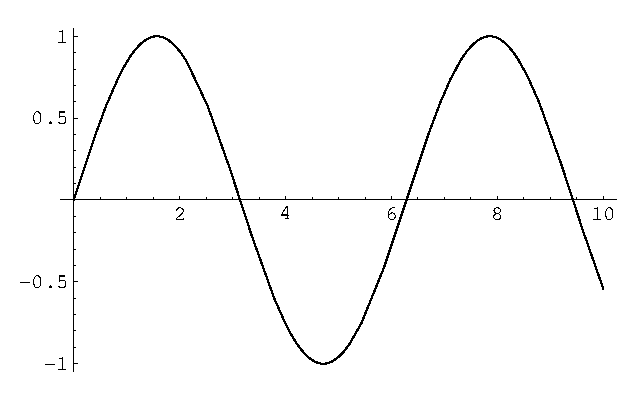
\includegraphics[width=5cm]{figures/mathematica}
\caption{Wykres.}\label{rys:plama}
\end{figure}

\begin{figure}[t]
\centering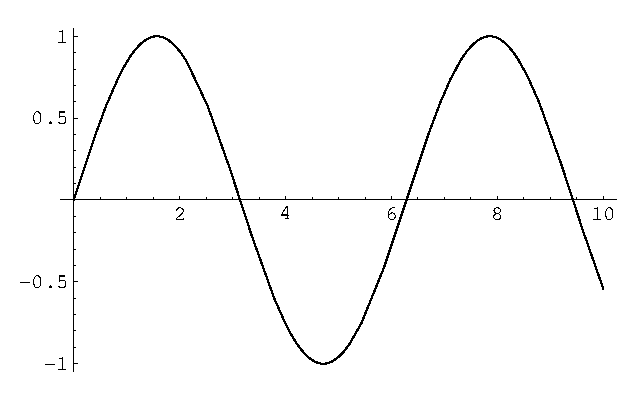
\includegraphics[width=\textwidth]{figures/mathematica}
\fcmfcaption{Ten sam wykres ale na szerokość tekstu. Formatowanie podpisu zgodne z wytycznymi FCMu.}\label{rys:plama2}
\end{figure}

Styl FCMu to nieco inne nagłówki rysunków. Dostepne są one poleceniem \texttt{fcmfcaption} (zob.~rysunek
\ref{rys:plama2}).

\subsection{Tablice}

Tablice to piękna rzecz, choć akurat ich umiejętne tworzenie w \LaTeX{}u nie jest łatwe. 
Jeśli tablica jest skomplikowana, to można ją na przykład wykonać w programie
OpenOffice, a następnie wyeksportować jako plik \akronim{PDF}. W każdym przypadku tablice wstawia się podobnie
jak rysunki, tylko że w środowisko \texttt{table}. Tradycja typograficzna sugeruje umieszczenie opisu tablicy, a więc
elementu \texttt{caption} ponad jej treścią (inaczej niż przy rysunkach).  

Tablica~\ref{tab:tabela} pokazuje pełen przykład.

\begin{table}[ht]
\caption{Przykładowa tabela. Styl opisu jest zgodny z rysunkami.}\label{tab:tabela}
\centering\footnotesize%
\begin{tabular}{l c}
\toprule
artykuł & cena [zł] \\
\midrule
bułka   & $0,4$ \\
masło   & $2,5$ \\
\bottomrule
\end{tabular}
\end{table}

Zasady FCMu sugerują nieco inne nagłówki tablic. Dostepne są one poleceniem \texttt{fcmtcaption} (zob.~tablicę
\ref{tab:tabela2}).

\begin{table}[ht]
\fcmtcaption{Przykładowa tabela. Styl opisu jest zgodny z wytycznymi FCMu.}\label{tab:tabela2}
\centering\footnotesize%
\begin{tabular}{l c}
\toprule
artykuł & cena [zł] \\
\midrule
bułka   & $0,4$ \\
masło   & $2,5$ \\
\bottomrule
\end{tabular}
\end{table}


\subsection{Checklista}

\begin{itemize}
\item Znakiem myślnika jest w LaTeXu dywiz pełen (---) albo półpauza (--), przykład:
  A niech to jasna cholera --- wrzasnąłem.

\item Połączenie między wyrazami to zwykły myślnik, przykład:   północno-zachodni

\item Sprawdź czy tutuł pracy ma maksymalnie dwa wiersze i czy stanowią one pełne frazy
  (czy nie ma przeniesienia bez sensu).

\item Sprawdź ostrzeżenia o 'overfull' i 'underful' boxes. Niektóre z nich można zignorować (spójrz
  na wynik formatowania), niektóre trzeba poprawić; czasem przeformułować zdanie.

item Przypisy stawia się wewnątrz zdań lub za kropką, przykład:
  Footnote is added after a comma.\footnote{Here is a footnote.}

\item Nie używaj przypisów zbyt często. Zobacz, czy nie lepiej będzie zintegrować przypis z tekstem.

\item Tytuły tabel, rysunków powinny kończyć się kropką.

\item Nie używaj modyfikatora [h] (here) do rysunków i tabel. Rysunki i tabele powinny być
  justowane do góry strony lub na stronie osobnej.

\item Wyróżnienie w tekście to polecenie \emph{wyraz}, nie należy używać czcionki pogrubionej (która
  wystaje wizualnie z tekstu i rozprasza).

\item Nazwy plików, katalogów, ścieżek, zmiennych środowiskowych, klas i metod formatujemy poleceniem
  \texttt{plik\_o\_pewnej\_nazwie}.

\item Po ostatniej zmianie do treści, sprawdź i przenieś wiszące spójniki wstawiając przed nie znak
  tyldy (twardej spacji), przykład:
  Ala i~kotek nie lubią mleczka, a~Stasiu lubi.
  
\item Za i.e. (id est) i e.g. (exempli gratia) stawia się zwyczajowo przecinek w typografii amerykańskiej.

\item Przed i za pełną pauza nie ma zwyczajowo spacji w typografii amerykańskiej, przykład:
  Darn, this looks good---said Mary.

\item Zamykający cudzysłów oraz footnote wychodzą za ostatni znak interpunkcji w typografii 
  amerykańskiej, przykłady:
  It can be called a ``curiosity,'' but it's actually normal.
  Footnote is added after a comma.\footnote{Here is a footnote.}

\item Odwołania do tabel i rysunków zawsze z wielkiej litery, przykład:
  In Figure~\ref{rys:plama} we illustrated XXX and in Table~\ref{tab:tabela} we show detailed data.
  
\end{itemize}


\section{Literatura i materiały dodatkowe}

Materiałów jest mnóstwo. Oto parę z nich:
\begin{itemize}
    \item \emph{The Not So Short Introduction\ldots}, która posiada również tłumaczenie 
    w języku polskim.\\
    \url{http://www.ctan.org/tex-archive/info/lshort/english/lshort.pdf}

    \item Klasy stylu \texttt{memoir} posiadają bardzo wiele informacji o składzie tekstów
    anglosaskich oraz sposoby dostosowania \LaTeX{}a do własnych potrzeb.\\
    \url{http://www.ctan.org/tex-archive/macros/latex/contrib/memoir/memman.pdf}
    
    \item Nasza grupa dyskusyjna i repozytorium Git są również dobrym miejscem aby zapytać
    (lub sprawdzić czy pytanie nie zostało już zadane).\\
    \url{https://github.com/politechnika/put-latex}

    \item Dla łaknących więcej wiedzy o systemie LaTeX podstawowym źródłem informacji
    jest książka Lamporta~\cite{Lamport1985}. Prawdziwy \emph{hardcore} to oczywiście
    \emph{The \TeX{}book} profesora Knutha~\cite{Knuth1986}.
\end{itemize}



%--------------------------------------
% Informacja o prawach autorskich
%--------------------------------------

\ppcolophon

\end{document}
